

\subsection{API REST de CloudNAO}
\label{\detokenize{chapter_two/desc_cloudnao:api-rest-de-cloudnao}}
Esta interfaz es el producto de la integración de modelos de aprendizaje
automático
enfocados a casos de uso relacionados con la robótica.
Es uno de los componentes más importantes en toda la arquitectura,
es el que une los servicios web de
terceros, los módulos mantenidos por el LAR y los entrega en una sola API.
Es un cliente y servidor a la vez.


\subsubsection{Descripción de la API}
\label{\detokenize{chapter_two/desc_cloudnao:documentacion-para-desarrolladores-clientes}}
La API REST de CloudNAO permite integrar dentro de una aplicación un
conjunto de herramientas para el análisis de imágenes.
Todas éstas basadas en modelos de aprendizaje automático. El URL base al
que todos los recursos son relativos es \sphinxcode{http://132.248.180.17/}.

La API tiene tres recursos:
\begin{itemize}
\item {} 
\sphinxcode{/register}: para que un nuevo usuario se registre y pueda ocupar los otros recursos. Envía una dirección de correo y una contraseña.

\item {} 
\sphinxcode{/refreshtoken}: para que el usuario pueda obtener un nuevo token de acceso al enviar los datos con los que se registró.

\item {} 
\sphinxcode{/vision}: el recurso más importante. Se le solicita que haga procesamiento de imágenes.

\end{itemize}

\paragraph{Vision}
\label{\detokenize{chapter_two/desc_cloudnao:vision}}
Este recurso es el encargado de la detección de características en una
imagen. Estas características son: la \sphinxstylestrong{detección de objetos}, el
\sphinxstylestrong{reconocimiento de rostros}, de personas previamente guardadas o de
nuevos sujetos para su almacenamiento, la \sphinxstylestrong{clasificación en cuatro escenarios}, lugares
dentro del laboratorio de algoritmos para la robótica, la
\sphinxstylestrong{detección de etiquetas o categorías}
y la \sphinxstylestrong{traducción de texto encontrado en una imagen}.

En este recurso la única forma de persistencia de datos es al guardar el
rostro de una nueva persona para su posterior reconocimiento.


\texttt{POST /vision}
\label{\detokenize{chapter_two/desc_cloudnao:post-vision}}\\

Se envía una imagen ya sea codificada en base 64 o mediante su URL y
las características que se desean obtener. Las características disponibles
son las siguientes:

\begin{itemize}
    \item{}
    \sphinxcode{FACE\_ENROLL}:
Detecta un rostro en la imagen y
con un identificador enviado en
el cuerpo de la petición se
almacena en una galería de
Kairos. Se emplea
\sphinxhref{https://www.kairos.com/docs/api/\#post-enroll}{/enroll}
de Kairos.
\item{}
\sphinxcode{FACE\_RECOGNITION}:
Encuentra rostros dentro de una
imagen y los relaciona con los
rostros similares previamente
guardados en una galería de
Kairos. Usa
\sphinxhref{https://www.kairos.com/docs/api/\#post-recognize}{/recognize}
de la API de Kairos.
\item{}
\sphinxcode{OBJECT\_DETECTION}:
Busca objetos en una la imagen,
usa la API de \sphinxhref{https://github.com/tensorflow/models/tree/master/research/object\_detection}{Tensorflow object
detection}.
Regresa las coordenadas de un
cuadro delimitador para cada
objeto detectado.
\item{}
\sphinxcode{LABELS\_DETECTION}:
Clasifica una imagen en distintas
categorías. Se vale de la API de
\sphinxhref{https://cloud.google.com/vision/docs/detecting-labels}{Google Cloud
Vision}
\item{}
\sphinxcode{OCR\_TRANSLATION}:
Lleva a cabo el reconocimiento de
texto en una imagen, para
posteriormente traducirlo.
Utiliza la API de \sphinxhref{https://cloud.google.com/vision/docs/ocr}{Google Cloud
Vision}
para el reconocimiento de
caracteres y la de \sphinxhref{https://cloud.google.com/translate/?hl=es}{Google Cloud
Translation}
para la segunda parte del proceso.
\item{}
\sphinxcode{CLASSIFY\_INDOOR\_SCENES}:
Clasifica una imagen en cuatro
categorías. Cada categoría es un
lugar dentro del área del LAR.

\end{itemize}


\subparagraph{Solicitud}
\label{\detokenize{chapter_two/desc_cloudnao:peticion}}

\subparagraph{Headers.}
\label{\detokenize{chapter_two/desc_cloudnao:headers}}
En los encabezados de la petición debe de ir el tipo de contenido que se envía
y un token de acceso único para cada usuario registrado. Esto último
simplemente es para evitar que cualquiera pueda hacer peticiones a la API.

\begin{sphinxVerbatim}[commandchars=\\\{\}]
\PYG{n}{Content}\PYG{o}{\PYGZhy{}}\PYG{n}{Type}\PYG{p}{:} \PYG{n}{application}\PYG{o}{/}\PYG{n}{json}
\PYG{n}{Authorization}\PYG{p}{:} \PYG{n}{ACCESS\PYGZus{}TOKEN}
\end{sphinxVerbatim}


\subparagraph{\sphinxstylestrong{Cuerpo.}}
\label{\detokenize{chapter_two/desc_cloudnao:body}}
En el cuerpo del mensaje se envía un JSON con la siguiente estructura. En la tabla 
\ref{tab:body_json_schema_request} se describen los atributos del JSON.

\begin{sphinxVerbatim}[commandchars=\\\{\}]
\PYG{p}{\PYGZob{}}
  \PYG{l+s+s2}{\PYGZdq{}imageContent\PYGZdq{}}\PYG{o}{:} \PYG{l+s+s2}{\PYGZdq{}Hello, world!\PYGZdq{}}\PYG{p}{,}
  \PYG{l+s+s2}{\PYGZdq{}imageSource\PYGZdq{}}\PYG{o}{:} \PYG{l+s+s2}{\PYGZdq{}Hello, world!\PYGZdq{}}\PYG{p}{,}
  \PYG{l+s+s2}{\PYGZdq{}features\PYGZdq{}}\PYG{o}{:} \PYG{p}{[}
    \PYG{p}{\PYGZob{}}
      \PYG{l+s+s2}{\PYGZdq{}type\PYGZdq{}}\PYG{o}{:} \PYG{l+s+s2}{\PYGZdq{}Hello, world!\PYGZdq{}}\PYG{p}{,}
      \PYG{l+s+s2}{\PYGZdq{}subjectID\PYGZdq{}}\PYG{o}{:} \PYG{l+s+s2}{\PYGZdq{}Hello, world!\PYGZdq{}}
    \PYG{p}{\PYGZcb{}}
  \PYG{p}{]}
\PYG{p}{\PYGZcb{}}
\end{sphinxVerbatim}


\begin{table}[h!]
\caption{Descripción del los elementos del JSON del cuerpo de la solicitud.\label{tab:body_json_schema_request}}
\begin{tabular}{|l|l}
\hline
\multicolumn{2}{|l|}{\textbf{Propiedades}}                                                                                                                                                                                                      \\ \hline
\multicolumn{2}{|l|}{imageContent}                                                                                                                                                                                                              \\ \hline
Tipo de dato & \multicolumn{1}{l|}{string}                                                                                                                                                                                                      \\ \hline
Descripción  & \multicolumn{1}{l|}{Imagen codificada en base 64.}                                                                                                                                                                               \\ \hline
\multicolumn{2}{|l|}{imageSource}                                                                                                                                                                                                               \\ \hline
Tipo de dato & \multicolumn{1}{l|}{string}                                                                                                                                                                                                      \\ \hline
Descripción  & \multicolumn{1}{l|}{URL pública de la imagen.}                                                                                                                                                                                   \\ \hline
\multicolumn{2}{|l|}{features}                                                                                                                                                                                                                  \\ \hline
Tipo de dato & \multicolumn{1}{l|}{array}                                                                                                                                                                                                       \\ \hline
\multirow{4}{*}{Descripción}  & 
\multicolumn{1}{l|}{
Una arreglo de las características que se desean detectar
en la} \\
&
\multicolumn{1}{l|}{imagen. Se debe solicitar al menos una de las seis disponibles.} \\&
\multicolumn{1}{l|}{Por ejemplo FACE\_ENROLL, FACE\_RECOGNITION,} \\& 
\multicolumn{1}{l|}{CLASSIFY\_INDOOR\_SCENES, etc.}


\\ \hline
\multicolumn{2}{|l|}{\textbf{Campos obligatorios}}                                                                                                                                                                                              \\ \hline
\multicolumn{2}{|l|}{imageContent}                                                                                                                                                                                                              \\
\multicolumn{2}{|l|}{imageSource}                                                                                                                                                                                                               \\
\multicolumn{2}{|l|}{features}                                                                                                                                                                                                                  \\ \hline
\end{tabular}
\end{table}



% \begin{sphinxVerbatim}[commandchars=\\\{\}]
% \PYG{p}{\PYGZob{}}
%   \PYG{l+s+s2}{\PYGZdq{}\PYGZdl{}schema\PYGZdq{}}\PYG{o}{:} \PYG{l+s+s2}{\PYGZdq{}http://json\PYGZhy{}schema.org/draft\PYGZhy{}04/schema\PYGZsh{}\PYGZdq{}}\PYG{p}{,}
%   \PYG{l+s+s2}{\PYGZdq{}type\PYGZdq{}}\PYG{o}{:} \PYG{l+s+s2}{\PYGZdq{}object\PYGZdq{}}\PYG{p}{,}
%   \PYG{l+s+s2}{\PYGZdq{}properties\PYGZdq{}}\PYG{o}{:} \PYG{p}{\PYGZob{}}
%     \PYG{l+s+s2}{\PYGZdq{}imageContent\PYGZdq{}}\PYG{o}{:} \PYG{p}{\PYGZob{}}
%       \PYG{l+s+s2}{\PYGZdq{}type\PYGZdq{}}\PYG{o}{:} \PYG{l+s+s2}{\PYGZdq{}string\PYGZdq{}}\PYG{p}{,}
%       \PYG{l+s+s2}{\PYGZdq{}description\PYGZdq{}}\PYG{o}{:} \PYG{l+s+s2}{\PYGZdq{}Imagen codificada en base 64\PYGZdq{}}
%     \PYG{p}{\PYGZcb{}}\PYG{p}{,}
%     \PYG{l+s+s2}{\PYGZdq{}imageSource\PYGZdq{}}\PYG{o}{:} \PYG{p}{\PYGZob{}}
%       \PYG{l+s+s2}{\PYGZdq{}type\PYGZdq{}}\PYG{o}{:} \PYG{l+s+s2}{\PYGZdq{}string\PYGZdq{}}\PYG{p}{,}
%       \PYG{l+s+s2}{\PYGZdq{}description\PYGZdq{}}\PYG{o}{:} \PYG{l+s+s2}{\PYGZdq{}URL de la imagen\PYGZdq{}}
%     \PYG{p}{\PYGZcb{}}\PYG{p}{,}
%     \PYG{l+s+s2}{\PYGZdq{}features\PYGZdq{}}\PYG{o}{:} \PYG{p}{\PYGZob{}}
%       \PYG{l+s+s2}{\PYGZdq{}type\PYGZdq{}}\PYG{o}{:} \PYG{l+s+s2}{\PYGZdq{}array\PYGZdq{}}\PYG{p}{,}
%       \PYG{l+s+s2}{\PYGZdq{}description\PYGZdq{}}\PYG{o}{:} \PYG{l+s+s2}{\PYGZdq{}Una arreglo de las características que se desean detectar en la imagen. Se debe solicitar al menos una de las seis disponibles. Por ejemplo FACE\PYGZus{}ENROLL, FACE\PYGZus{}RECOGNITION, CLASSIFY\PYGZus{}INDOOR\PYGZus{}SCENES, etc.\PYGZdq{}}
%     \PYG{p}{\PYGZcb{}}
%   \PYG{p}{\PYGZcb{}}\PYG{p}{,}
%   \PYG{l+s+s2}{\PYGZdq{}required\PYGZdq{}}\PYG{o}{:} \PYG{p}{[}
%     \PYG{l+s+s2}{\PYGZdq{}imageContent\PYGZdq{}}\PYG{p}{,}
%     \PYG{l+s+s2}{\PYGZdq{}imageSource\PYGZdq{}}\PYG{p}{,}
%     \PYG{l+s+s2}{\PYGZdq{}features\PYGZdq{}}
%   \PYG{p}{]}
% \PYG{p}{\PYGZcb{}}
% \end{sphinxVerbatim}


\subparagraph{\sphinxstylestrong{Respuesta}}
\label{\detokenize{chapter_two/desc_cloudnao:respuesta}}

\subparagraph{\sphinxstylestrong{Cuepo.}}
\label{\detokenize{chapter_two/desc_cloudnao:id1}}
En el cuerpo del mensaje de respuesta si se obtiene un código 200
se obtiene un JSON con las características encontradas. En éste también
se incluyen mensajes de error que no pertencen al estándar del protocolo HTTP.
En la tabla \ref{tab:json_schema_response} se describen los atributos del JSON.

\begin{sphinxVerbatim}[commandchars=\\\{\}]
\PYG{p}{\PYGZob{}}
  \PYG{l+s+s2}{\PYGZdq{}features\PYGZdq{}}\PYG{o}{:} \PYG{p}{\PYGZob{}}
    \PYG{l+s+s2}{\PYGZdq{}faceRecognition\PYGZdq{}}\PYG{o}{:} \PYG{p}{[}
      \PYG{p}{\PYGZob{}}
        \PYG{l+s+s2}{\PYGZdq{}topLeftX\PYGZdq{}}\PYG{o}{:} \PYG{l+m+mi}{1}\PYG{p}{,}
        \PYG{l+s+s2}{\PYGZdq{}topLeftY\PYGZdq{}}\PYG{o}{:} \PYG{l+m+mi}{1}\PYG{p}{,}
        \PYG{l+s+s2}{\PYGZdq{}width\PYGZdq{}}\PYG{o}{:} \PYG{l+m+mi}{1}\PYG{p}{,}
        \PYG{l+s+s2}{\PYGZdq{}height\PYGZdq{}}\PYG{o}{:} \PYG{l+m+mi}{1}\PYG{p}{,}
        \PYG{l+s+s2}{\PYGZdq{}subjectId\PYGZdq{}}\PYG{o}{:} \PYG{l+s+s2}{\PYGZdq{}Hello, world!\PYGZdq{}}\PYG{p}{,}
        \PYG{l+s+s2}{\PYGZdq{}confidence\PYGZdq{}}\PYG{o}{:} \PYG{l+m+mi}{1}
      \PYG{p}{\PYGZcb{}}
    \PYG{p}{]}\PYG{p}{,}
    \PYG{l+s+s2}{\PYGZdq{}objectDetection\PYGZdq{}}\PYG{o}{:} \PYG{p}{[}
      \PYG{p}{\PYGZob{}}
        \PYG{l+s+s2}{\PYGZdq{}category\PYGZdq{}}\PYG{o}{:} \PYG{l+s+s2}{\PYGZdq{}Hello, world!\PYGZdq{}}\PYG{p}{,}
        \PYG{l+s+s2}{\PYGZdq{}confidence\PYGZdq{}}\PYG{o}{:} \PYG{l+m+mi}{1}\PYG{p}{,}
        \PYG{l+s+s2}{\PYGZdq{}topLeftX\PYGZdq{}}\PYG{o}{:} \PYG{l+m+mi}{1}\PYG{p}{,}
        \PYG{l+s+s2}{\PYGZdq{}topLeftY\PYGZdq{}}\PYG{o}{:} \PYG{l+m+mi}{1}\PYG{p}{,}
        \PYG{l+s+s2}{\PYGZdq{}width\PYGZdq{}}\PYG{o}{:} \PYG{l+m+mi}{1}\PYG{p}{,}
        \PYG{l+s+s2}{\PYGZdq{}height\PYGZdq{}}\PYG{o}{:} \PYG{l+m+mi}{1}
      \PYG{p}{\PYGZcb{}}
    \PYG{p}{]}\PYG{p}{,}
    \PYG{l+s+s2}{\PYGZdq{}labelsDetection\PYGZdq{}}\PYG{o}{:} \PYG{p}{[}
      \PYG{p}{\PYGZob{}}
        \PYG{l+s+s2}{\PYGZdq{}name\PYGZdq{}}\PYG{o}{:} \PYG{l+s+s2}{\PYGZdq{}Hello, world!\PYGZdq{}}\PYG{p}{,}
        \PYG{l+s+s2}{\PYGZdq{}confidence\PYGZdq{}}\PYG{o}{:} \PYG{l+m+mi}{1}
      \PYG{p}{\PYGZcb{}}
    \PYG{p}{]}\PYG{p}{,}
    \PYG{l+s+s2}{\PYGZdq{}ocrTranslation\PYGZdq{}}\PYG{o}{:} \PYG{p}{\PYGZob{}}
      \PYG{l+s+s2}{\PYGZdq{}sourceText\PYGZdq{}}\PYG{o}{:} \PYG{l+s+s2}{\PYGZdq{}Hello, world!\PYGZdq{}}\PYG{p}{,}
      \PYG{l+s+s2}{\PYGZdq{}targetText\PYGZdq{}}\PYG{o}{:} \PYG{l+s+s2}{\PYGZdq{}Hello, world!\PYGZdq{}}\PYG{p}{,}
      \PYG{l+s+s2}{\PYGZdq{}sourceLanguage\PYGZdq{}}\PYG{o}{:} \PYG{l+s+s2}{\PYGZdq{}Hello, world!\PYGZdq{}}
    \PYG{p}{\PYGZcb{}}\PYG{p}{,}
    \PYG{l+s+s2}{\PYGZdq{}faceEnroll\PYGZdq{}}\PYG{o}{:} \PYG{p}{\PYGZob{}}
      \PYG{l+s+s2}{\PYGZdq{}topLeftX\PYGZdq{}}\PYG{o}{:} \PYG{l+m+mi}{1}\PYG{p}{,}
      \PYG{l+s+s2}{\PYGZdq{}topLeftY\PYGZdq{}}\PYG{o}{:} \PYG{l+m+mi}{1}\PYG{p}{,}
      \PYG{l+s+s2}{\PYGZdq{}width\PYGZdq{}}\PYG{o}{:} \PYG{l+m+mi}{1}\PYG{p}{,}
      \PYG{l+s+s2}{\PYGZdq{}height\PYGZdq{}}\PYG{o}{:} \PYG{l+m+mi}{1}\PYG{p}{,}
      \PYG{l+s+s2}{\PYGZdq{}confidence\PYGZdq{}}\PYG{o}{:} \PYG{l+m+mi}{1}\PYG{p}{,}
      \PYG{l+s+s2}{\PYGZdq{}gender\PYGZdq{}}\PYG{o}{:} \PYG{l+s+s2}{\PYGZdq{}Hello, world!\PYGZdq{}}
    \PYG{p}{\PYGZcb{}}
    \PYG{l+s+s2}{\PYGZdq{}indoorScenesClassify\PYGZdq{}} \PYG{o}{:} \PYG{p}{\PYGZob{}}
      \PYG{l+s+s2}{\PYGZdq{}indoorScene\PYGZdq{}}\PYG{o}{:} \PYG{l+s+s2}{\PYGZdq{}Hello, world!\PYGZdq{}}
    \PYG{p}{\PYGZcb{}}
  \PYG{p}{\PYGZcb{}}\PYG{p}{,}
\PYG{p}{\PYGZcb{}}
\end{sphinxVerbatim}

\begin{longtable}{|l|l|}
\caption{Atributos que componen el JSON del cuerpo de la respuesta.\label{tab:json_schema_response}}\\
\hline
\multicolumn{2}{|l|}{\cellcolor[HTML]{68CBD0}\texttt{features}}                                                                                                                                \\ \hline
\endfirsthead
%
\endhead
%
\cellcolor[HTML]{68CBD0}\textbf{Tipo de dato} & objeto                                                                                                                                         \\ \hline
\multicolumn{2}{|l|}{\cellcolor[HTML]{68CBD0}\textbf{Propiedades}}                                                                                                                             \\ \hline
\multicolumn{2}{|l|}{\cellcolor[HTML]{68CBD0}\texttt{faceRecognition}}                                                                                                                         \\ \hline
Tipo de dato                                  & array                                                                                                                                          \\ \hline
Descripción                                   & \begin{tabular}[c]{@{}l@{}}Un arreglo de objetos que contienen \\ a los rostros reconocidos.\end{tabular}                                      \\ \hline
\multicolumn{2}{|l|}{\cellcolor[HTML]{68CBD0}\texttt{objectDetection}}                                                                                                                         \\ \hline
Tipo de dato                                  & array                                                                                                                                          \\ \hline
Descripción                                   & Contiene un arreglo con todos los objetos detectados.                                                                                          \\ \hline
\multicolumn{2}{|l|}{\cellcolor[HTML]{68CBD0}\texttt{labelsDetection}}                                                                                                                         \\ \hline
Tipo de dato                                  & array                                                                                                                                          \\ \hline
Descripción                                   & Contiene un arreglo con las etiquetas de la imagen.                                                                                            \\ \hline
\multicolumn{2}{|l|}{\cellcolor[HTML]{68CBD0}\texttt{ocrTranslation}}                                                                                                                          \\ \hline
\cellcolor[HTML]{FFFFFF}Tipo de dato          & objeto                                                                                                                                         \\ \hline
\multicolumn{2}{|l|}{\cellcolor[HTML]{FFFFFF}Propiedades}                                                                                                                                      \\ \hline
\multicolumn{2}{|l|}{\texttt{sourceText}}                                                                                                                                                      \\ \hline
Tipo de dato                                  & string                                                                                                                                         \\ \hline
Descripción                                   & El texto en formato UTF-8.                                                                                                                     \\ \hline
\multicolumn{2}{|l|}{\texttt{targetText}}                                                                                                                                                      \\ \hline
Tipo de dato                                  & string                                                                                                                                         \\ \hline
Descripción                                   & El texto traducido.                                                                                                                            \\ \hline
\multicolumn{2}{|l|}{\texttt{sourceLanguage}}                                                                                                                                                  \\ \hline
Tipo de dato                                  & string                                                                                                                                         \\ \hline
Descripción                                   & El idioma original.                                                                                                                            \\ \hline
Descripción                                   & Un objecto con el texto encontrado en la imagen.                                                                                               \\ \hline
\multicolumn{2}{|l|}{\cellcolor[HTML]{68CBD0}\texttt{faceEnroll}}                                                                                                                              \\ \hline
Tipo de dato                                  & objeto                                                                                                                                         \\ \hline
\multicolumn{2}{|l|}{Propiedades}                                                                                                                                                              \\ \hline
\multicolumn{2}{|l|}{\texttt{topLeftX}}                                                                                                                                                        \\ \hline
Tipo de dato                                  & number                                                                                                                                         \\ \hline
Descripción                                   & Coordenada sobre el eje x.                                                                                                                     \\ \hline
\multicolumn{2}{|l|}{\texttt{topLeftY}}                                                                                                                                                        \\ \hline
Tipo de dato                                  & number                                                                                                                                         \\ \hline
Descripción                                   & Coordenada                                                                                                                                     \\ \hline
\multicolumn{2}{|l|}{\texttt{width}}                                                                                                                                                           \\ \hline
Tipo de dato                                  & number                                                                                                                                         \\ \hline
Descripción                                   & Ancho del recuadro que delimita la imagen.                                                                                                     \\ \hline
\multicolumn{2}{|l|}{\texttt{height}}                                                                                                                                                          \\ \hline
Tipo de dato                                  & number                                                                                                                                         \\ \hline
Descripción                                   & Altura del recuadro que delimita la imagen.                                                                                                    \\ \hline
\multicolumn{2}{|l|}{\texttt{confidence}}                                                                                                                                                      \\ \hline
Tipo de dato                                  & number                                                                                                                                         \\ \hline
Descripción                                   & Valor de 0-1 que representa una probabilidad.                                                                                                  \\ \hline
\multicolumn{2}{|l|}{\texttt{gender}}                                                                                                                                                          \\ \hline
Tipo de dato                                  & string                                                                                                                                         \\ \hline
Descripción                                   & Sexo de la persona con ese rostro (M o F)                                                                                                      \\ \hline
Descripción                                   & Características del rostro detectado.                                                                                                          \\ \hline
\multicolumn{2}{|l|}{\cellcolor[HTML]{68CBD0}\texttt{indoorScenesClassify}}                                                                                                                    \\ \hline
Tipo de dato                                  & objeto                                                                                                                                         \\ \hline
\multicolumn{2}{|l|}{Propiedades}                                                                                                                                                              \\ \hline
\multicolumn{2}{|l|}{\texttt{indoorScene}}                                                                                                                                                     \\ \hline
Tipo de dato                                  & string                                                                                                                                         \\ \hline
Descripción                                   & \begin{tabular}[c]{@{}l@{}}La escena detectada, puede ser cualquiera de las\\ cuatro posibles \(exit, soccer_court, desks, office\)\end{tabular} \\ \hline
Descripción                                   & Escenario reconocido.                                                                                                                          \\ \hline
\cellcolor[HTML]{68CBD0}\textbf{Descripción}  & \begin{tabular}[c]{@{}l@{}}Lista con las respuestas de acuerdo a las \\ características que se solicitaron.\end{tabular}                       \\ \hline
\end{longtable}


\subparagraph{Ejemplo de una petición a la API con CURL}



\subsubsection{Guía para desarrolladores}
\label{\detokenize{chapter_two/desc_cloudnao:documentacion-para-maintainers-de-la-api}}
Esta API puede funcionar de manera individual, no es necesario contar con todos
los componentes de la arquitectura. Puede integrarse en algún otro sistema,
donde se requieran los mismos servicios web. 

Está desarrollada en el lenguaje de programación Python, utilizando el framework
Flask. La siguiente lista muestra las dependencias más importantes:
\begin{itemize}
\item {} 
\sphinxstylestrong{Flask}, un microframework para desarrollar aplicaciones web, y extensiones de éste como:
\begin{itemize}
\item {} 
\sphinxstylestrong{Flask-RESTful}, para contruir rápidamente una API REST.

\item {} 
\sphinxstylestrong{Flask-SQLAlchemy}, Es una biblioteca que implementa la técnica ORM (Mapeador Relacional de Objetos), la cual permite consultar y manipular datos de una base de datos usando el paradigma orientado a objetos.

\item {} 
\sphinxstylestrong{Flask-Script}, una interfaz la línea de comandos.

\end{itemize}

\item {} 
\sphinxstylestrong{Tensorflow},  una biblioteca de código abierto para cómputo numérico usando gráficas de flujos de datos.

\item {} 
\sphinxstylestrong{numpy}, una biblioteca para cómputo científico.

\item {} 
\sphinxstylestrong{requests}, una biblioteca para las peticiones HTTP a servicios web.

\end{itemize}

Para comprender mejor este elemento, en las siguientes subsecciones se describen
cada una de las herramientas utilizadas, primero el framework Flask, junto con
sus extensiones y las otras bibliotecas mencionadas. Después explico su
integración en una sola aplicación, y finalmente las opciones de
configuración e instalación, así como su despliegue en un servidor.


\paragraph{Flask}
\label{\detokenize{chapter_two/desc_cloudnao:flask}}

Flask es un micro framework para desarrollo web. Fue diseñado para ser un
framework extensible, sólo provee un núcleo sólido con servicios básicos,
mientras que las extensiones brindan el resto. Esto quiere decir que Flask,
te da la posibilidad de como desarrollador contar sólo con las dependecias que
necesitas.

Tiene dos dependecias principales, \sphinxstylestrong{Werkzeug} y \sphinxstylestrong{Jinja2}.
El enrutamiento, debugging y WSGI tienen procedencia de Werkzeug.
Jinga2 ofrece el soporte para el manejo de plantillas. Para nuestra
aplicación solamente hacemos uso de la primera.
\begin{quote}

\sphinxstyleemphasis{WSGI} es la Web Server Gateway Interface. Es un protocolo que describe
cómo un servido web se comunica con aplicaciones web, y cómo las aplicaciones
web se pueden encadenar para procesar una petición.
\end{quote}

Para la instalación de Flask así como de cualquier paquete de Python, se
recomienda crear un ambiente virtual con la herramienta \sphinxstylestrong{virtualenv}
Un ambiente virtual es una copia privada del intérprete de Python sobre la cual
es posible instalar paquetes de manera privada, sin afectar al intérprete
global de Python. Permite crear un ambiente de trabajo aislado para cada
proyecto, así cada aplicación tiene acceso solo a los paquetes que utiliza.

Con esto, todo lo descrito a continuación que se refiera a la instalación de
paquetes o ejecución de programas se hace dentro de un ambiente virtual.


\subparagraph{Inicialización.}
\label{\detokenize{chapter_two/desc_cloudnao:inicializacion}}
Todas las aplicaciones de Flask deben crear una \sphinxstyleemphasis{instacia de la aplicación}. Este
objeto maneja todas las peticiones que recibe el servidor web, usando
la especificación WSGI.
La instancia de la aplicación es un objeto de la clase Flask,
se crea de la siguiente manera:

\begin{sphinxVerbatim}[commandchars=\\\{\}]
\PYG{k+kn}{from} \PYG{n+nn}{flask} \PYG{k}{import} \PYG{n}{Flask}
\PYG{n}{app} \PYG{o}{=} \PYG{n}{Flask}\PYG{p}{(}\PYG{n+nv+vm}{\PYGZus{}\PYGZus{}name\PYGZus{}\PYGZus{}}\PYG{p}{)}
\end{sphinxVerbatim}

El único argumento requerido para el contructor de la clase Flask es el nombre
del módulo o paquete de la aplicación. Para la mayoría de los casos,
la variable de Python \sphinxcode{\_\_name\_\_} es el valor correcto. Flask usa este argumento
para determinar la ruta raíz de la aplicación, para que después pueda encontrar
los archivos de los recursos relativos a la ubicación de la aplicación.


\subparagraph{Rutas.}
\label{\detokenize{chapter_two/desc_cloudnao:rutas}}
Los clientes envían peticiones al servidor web, que a su vez las envía a la
instancia de la aplicación de Flask. La instacia de la aplicación necesita saber
qué código debe regresar para cada URL solicitado, así que mantiene un mapeo de
los URL a funciones de Python. La asociación entre el URL y la función que se
la maneja se llama \sphinxstyleemphasis{ruta}.

La manera más conveniente de definir una ruta en una aplicación de Flask es
a través del decorador \sphinxcode{app.route}, que registra la función decorada como
una ruta.

El siguiente ejemplo registra la función \sphinxcode{index()} como el manejador para el URL
raíz de la aplicación. Si la aplicación fue desplegada en un servidor con el
nombre del dominio \sphinxurl{http://www.lar.com}. Al acceder desde un navegador a
la dirección anterior se ejecutará la función \sphinxcode{index()} del lado del servidor.
El valor
retornado por esta función se llama \sphinxstyleemphasis{respuesta}, y es lo que el cliente recibe.
Las funciones como \sphinxcode{index()} se llaman \sphinxstyleemphasis{funciones de vista}.
En este caso el navegador mostrará \sphinxcode{Hola mundo}.

\begin{sphinxVerbatim}[commandchars=\\\{\}]
\PYG{n+nd}{@app}\PYG{o}{.}\PYG{n}{route}\PYG{p}{(}\PYG{l+s+s1}{\PYGZsq{}}\PYG{l+s+s1}{/}\PYG{l+s+s1}{\PYGZsq{}}\PYG{p}{)}
\PYG{k}{def} \PYG{n+nf}{index}\PYG{p}{(}\PYG{p}{)}\PYG{p}{:}
  \PYG{k}{return} \PYG{l+s+s2}{\PYGZdq{}}\PYG{l+s+s2}{Hola mundo}\PYG{l+s+s2}{\PYGZdq{}}
\end{sphinxVerbatim}

Flask soporta los tipos de URL con componentes dinámicos utilizando
una sintáxis especial en el decorador \sphinxcode{route}. En el siguiente ejemplo se
muestra el nombre de usuario como componente dinámico.

\begin{sphinxVerbatim}[commandchars=\\\{\}]
\PYG{n+nd}{@app}\PYG{o}{.}\PYG{n}{route}\PYG{p}{(}\PYG{l+s+s1}{\PYGZsq{}}\PYG{l+s+s1}{/usuario/\PYGZlt{}nombre\PYGZgt{}}\PYG{l+s+s1}{\PYGZsq{}}\PYG{p}{)}
\PYG{k}{def} \PYG{n+nf}{user}\PYG{p}{(}\PYG{n}{nombre}\PYG{p}{)}\PYG{p}{:}
  \PYG{k}{return} \PYG{l+s+s2}{\PYGZdq{}}\PYG{l+s+s2}{Hola, }\PYG{l+s+si}{\PYGZob{}\PYGZcb{}}\PYG{l+s+s2}{\PYGZdq{}}\PYG{o}{.}\PYG{n}{format}\PYG{p}{(}\PYG{n}{nombre}\PYG{p}{)}
\end{sphinxVerbatim}

La parte encerrada por los paréntesis angulares es el componente dinámico, así
que cualesquiera URL que coincidan con la porción estática será mapeada a esta
ruta.

El decorador \sphinxcode{app.route} cuenta con un argumento opcional \sphinxcode{methods},
el cual recibe
una lista de métodos HTTP. \sphinxcode{methods} le dice a Flask que registra a las
funciones de vista como manejadores para las peticiones de acuerdo
al tipo de método enviado. Cuando \sphinxcode{methods} no está el los parámetros de la
función, la función de vista es registrada para manejar solamente peticiones
\sphinxcode{GET}. El siguiente ejemplo se le pide a Flask que se registre a la
función de vista como manejadora de petición de tipo \sphinxcode{GET} y \sphinxcode{POST}.

\begin{sphinxVerbatim}[commandchars=\\\{\}]
\PYG{n+nd}{@app}\PYG{o}{.}\PYG{n}{route}\PYG{p}{(}\PYG{l+s+s1}{\PYGZsq{}}\PYG{l+s+s1}{/usuario/\PYGZlt{}nombre\PYGZgt{}}\PYG{l+s+s1}{\PYGZsq{}}\PYG{p}{,} \PYG{n}{methods}\PYG{o}{=}\PYG{p}{[}\PYG{l+s+s1}{\PYGZsq{}}\PYG{l+s+s1}{GET}\PYG{l+s+s1}{\PYGZsq{}}\PYG{p}{,} \PYG{l+s+s1}{\PYGZsq{}}\PYG{l+s+s1}{POST}\PYG{l+s+s1}{\PYGZsq{}}\PYG{p}{]}\PYG{p}{)}
\PYG{k}{def} \PYG{n+nf}{user}\PYG{p}{(}\PYG{n}{nombre}\PYG{p}{)}\PYG{p}{:}
  \PYG{k}{return} \PYG{l+s+s2}{\PYGZdq{}}\PYG{l+s+s2}{Hola, }\PYG{l+s+si}{\PYGZob{}\PYGZcb{}}\PYG{l+s+s2}{\PYGZdq{}}\PYG{o}{.}\PYG{n}{format}\PYG{p}{(}\PYG{n}{nombre}\PYG{p}{)}
\end{sphinxVerbatim}


\subparagraph{Arranque del servidor.}
\label{\detokenize{chapter_two/desc_cloudnao:arranque-del-servidor}}
La instancia de la aplicación tiene un tiene un método \sphinxcode{run} que inicia el
servidor web integrado con Flask, el cual sólo está destinado para usarse
durante el desarrollo.

\begin{sphinxVerbatim}[commandchars=\\\{\}]
\PYG{k}{if} \PYG{n+nv+vm}{\PYGZus{}\PYGZus{}name\PYGZus{}\PYGZus{}} \PYG{o}{==} \PYG{l+s+s1}{\PYGZsq{}}\PYG{l+s+s1}{\PYGZus{}\PYGZus{}main\PYGZus{}\PYGZus{}}\PYG{l+s+s1}{\PYGZsq{}}\PYG{p}{:}
  \PYG{n}{app}\PYG{o}{.}\PYG{n}{run}\PYG{p}{(}\PYG{n}{debug}\PYG{o}{=}\PYG{k+kc}{True}\PYG{p}{)}
\end{sphinxVerbatim}

Una vez que el servidor es puesto en marcha, entra en un bucle que espera por
peticiones para procesarlas. Este bucle continua hasta que la aplicación es
detenida.

Existen varios parámetros que \sphinxcode{app.run()} puede recibir para configurar el
modo de operación del servidor web. Durante el desarrollo, conviene  activar
el modo de debugging, que entre otras cosas activa el \sphinxstyleemphasis{debugger} y el \sphinxstyleemphasis{reloader}.
Esto se hace pasando el argumento \sphinxcode{debug} igual a \sphinxcode{True} .


% \subparagraph{El ciclo de Petición-Respuesta}
% \label{\detokenize{chapter_two/desc_cloudnao:el-ciclo-de-peticion-respuesta}}
% En las siguientes secciones se ahonda un poco en el diseño de diversos aspectos
% del framework


% \subparagraph{Los contextos de aplicación y de petición}
% \label{\detokenize{chapter_two/desc_cloudnao:los-contextos-de-aplicacion-y-de-peticion}}
% Cuando Flask recibe una petición desde un cliente, necesita hacer que la función
% de vista tenga disponibles algunos objetos de los que se encargará. Un ejemplo
% de estos es el objeto \sphinxstyleemphasis{request}, que encapsula la petición HTTP enviada
% por el cliente.

% Flask utiliza \sphinxstyleemphasis{contextos} para que ciertos objetos sean accesibles globalmente
% de manera temporal. Sin embargo, regresando al ejemplo del \sphinxcode{request}, éste no
% puede ser una variable global si consideras un servidor web con múltiples hilos,
% cada hilo trabaja con diferentes peticiones de clientes diferentes al mismo
% tiempo, así que cada hilo necesita un objeto \sphinxcode{request} diferente. Los
% contextos permiten que Flask haga ciertas variables accesibles globalmente en un
% hilo sin interferir con otros hilos.

% Hay dos contextos en Flask: el \sphinxstyleemphasis{contexto de aplicación y el de petición}.
% La \hyperref[\detokenize{chapter_two/desc_cloudnao:globals-contexts}]{Tabla \ref{\detokenize{chapter_two/desc_cloudnao:globals-contexts}}} muestra las variables de ambos contextos.


% \begin{savenotes}\sphinxattablestart
% \centering
% \sphinxcapstartof{table}
% \sphinxcaption{Contextos globales de Flask}\label{\detokenize{chapter_two/desc_cloudnao:globals-contexts}}
% \sphinxaftercaption
% \begin{tabulary}{\linewidth}[t]{|T|T|T|}
% \hline
% \sphinxstylethead{ 
% Nombre de la variable
% \unskip}\relax &\sphinxstylethead{ 
% Contexto
% \unskip}\relax &\sphinxstylethead{ 
% Descripción
% \unskip}\relax \\
% \hline
% \sphinxcode{current\_app{}`}
% &
% De aplicación
% &
% La instancia de la aplicación.
% \\
% \hline
% \sphinxcode{g}
% &
% De aplicación
% &
% Un objeto que la aplicación puede usar para almacenamiento temporal mientras maneja una petición. Esta variable se inicializa con cada petición.
% \\
% \hline
% \sphinxcode{request}
% &
% De petición
% &
% Encapsula el contenido de una petición HTTP enviada por el cliente.
% \\
% \hline
% \sphinxcode{session}
% &
% De petición
% &
% La sesión del usuario, un diccionario que la aplicación puede usar para guardar valores que se «recuerdan» entre peticiones.
% \\
% \hline
% \end{tabulary}
% \par
% \sphinxattableend\end{savenotes}


% \subparagraph{Hooks de peticiones}
% \label{\detokenize{chapter_two/desc_cloudnao:hooks-de-peticiones}}
% A veces es útil ejecutar código antes o después de que una petición sea
% procesada. Por ejemplo, para hacer la conexión a una base de datos o para
% autenticación de usuarios. Flask brinda la opción de registrar funciones que
% serán invocadas antes o después de que una petición sea enviada a una función
% de vista.

% Los hooks de peticiones están implementados como decoradores. Los siguientes son
% los cuatro soportados por Flask:
% \begin{itemize}
% \item {} 
% \sphinxcode{before\_first\_request}: Registra una función para que se ejecute antes de que la primera petición se maneje.

% \item {} 
% \sphinxcode{before\_request}: Registra una función para su ejecución antes de cada petición.

% \item {} 
% \sphinxcode{after\_request}: Registra una función para que corra después de cada petición, si no hay excepciones que no se hayan manejado.

% \item {} 
% \sphinxcode{teardown\_request}: Registra una función para ejecutarse después de cada petición, incluso si hay excepciones que no se hayan manejado.

% \end{itemize}


% \subparagraph{Respuestas}
% \label{\detokenize{chapter_two/desc_cloudnao:respuestas}}
% Cuando Flask invoca un función de vista, se espera que el valor retornado sea
% la respuesta de la petición. En la mayoría de los casos la respuesta es una
% cadena que se envía al cliente como una página HTML.

% Sin embargo, el protocolo HTTP necesita más que solo una cadena para enviar
% como respuesta.
% Una parte importante de una respuesta HTTP es el código de estado,
% Flask establece el código \sphinxcode{200} por defecto.

% Cuando una función de vista necesita responder con un código de estado diferente,
% puede añadirse un código numérico como segundo valor retornado después del
% texto de respuesta. El siguiente ejemplo muesta una función de vista que
% retorna un mensaje de error, y el código \sphinxcode{400}, mala petición.

% \begin{sphinxVerbatim}[commandchars=\\\{\}]
% \PYG{n+nd}{@app}\PYG{o}{.}\PYG{n}{route}\PYG{p}{(}\PYG{l+s+s1}{\PYGZsq{}}\PYG{l+s+s1}{/}\PYG{l+s+s1}{\PYGZsq{}}\PYG{p}{)}
% \PYG{k}{def} \PYG{n+nf}{index}\PYG{p}{(}\PYG{p}{)}\PYG{p}{:}
%   \PYG{k}{return} \PYG{l+s+s2}{\PYGZdq{}}\PYG{l+s+s2}{Bad Request}\PYG{l+s+s2}{\PYGZdq{}}\PYG{p}{,} \PYG{l+m+mi}{400}
% \end{sphinxVerbatim}

% En vez de retornar una tupla con varios valores, la funciones de vista tienen
% la opción de regresar un objeto \sphinxcode{Response}. La función \sphinxcode{make\_response()}
% recibe uno, dos o tres argumentos, los mismos valores que pueden ser regresados
% por una función de vista, y retorna un objeto \sphinxcode{Response}. El siguiente ejemplo
% crea un objeto respuesta y añade una cookie en él:

% \begin{sphinxVerbatim}[commandchars=\\\{\}]
% \PYG{k+kn}{from} \PYG{n+nn}{flask} \PYG{k}{import} \PYG{n}{make\PYGZus{}response}
% \PYG{n+nd}{@app}\PYG{o}{.}\PYG{n}{route}\PYG{p}{(}\PYG{l+s+s1}{\PYGZsq{}}\PYG{l+s+s1}{/}\PYG{l+s+s1}{\PYGZsq{}}\PYG{p}{)}
% \PYG{k}{def} \PYG{n+nf}{index}\PYG{p}{(}\PYG{p}{)}\PYG{p}{:}
%   \PYG{n}{response} \PYG{o}{=} \PYG{n}{make\PYGZus{}response}\PYG{p}{(}\PYG{l+s+s2}{\PYGZdq{}}\PYG{l+s+s2}{Este documento tiene una cookie}\PYG{l+s+s2}{\PYGZdq{}}\PYG{p}{)}
%   \PYG{n}{response}\PYG{o}{.}\PYG{n}{set\PYGZus{}cookie}\PYG{p}{(}\PYG{l+s+s2}{\PYGZdq{}}\PYG{l+s+s2}{respuesta}\PYG{l+s+s2}{\PYGZdq{}}\PYG{p}{,} \PYG{l+s+s2}{\PYGZdq{}}\PYG{l+s+s2}{42}\PYG{l+s+s2}{\PYGZdq{}}\PYG{p}{)}
%   \PYG{k}{return} \PYG{n}{response}
% \end{sphinxVerbatim}

% Existe un tipo de respuesta especial llamado \sphinxstyleemphasis{redirección}. Esta respuesta no
% incluye la página de un documento; sólo da al navergador una URL de la cual
% debe cargar una nueva página.

% \begin{sphinxVerbatim}[commandchars=\\\{\}]
% \PYG{k+kn}{from} \PYG{n+nn}{flask} \PYG{k}{import} \PYG{n}{redirect}
% \PYG{n+nd}{@app}\PYG{o}{.}\PYG{n}{route}\PYG{p}{(}\PYG{l+s+s1}{\PYGZsq{}}\PYG{l+s+s1}{/}\PYG{l+s+s1}{\PYGZsq{}}\PYG{p}{)}
% \PYG{k}{def} \PYG{n+nf}{index}\PYG{p}{(}\PYG{p}{)}\PYG{p}{:}
%   \PYG{k}{return} \PYG{n}{redirect}\PYG{p}{(}\PYG{l+s+s1}{\PYGZsq{}}\PYG{l+s+s1}{http://www.google.com}\PYG{l+s+s1}{\PYGZsq{}}\PYG{p}{)}
% \end{sphinxVerbatim}

% Otra respuesta especial es emitida por la función \sphinxcode{abort}, que se usa para
% el manejo de errores. El ejemplo mostrado a continuación retorna el código
% de estado \sphinxcode{404} si el componente dinámico en el URL no representa un usuario
% válido:

% \begin{sphinxVerbatim}[commandchars=\\\{\}]
% \PYG{k+kn}{from} \PYG{n+nn}{flask} \PYG{k}{import} \PYG{n}{abort}
% \PYG{n}{users} \PYG{o}{=} \PYG{p}{\PYGZob{}}
%     \PYG{l+s+s2}{\PYGZdq{}}\PYG{l+s+s2}{N7FAA52317}\PYG{l+s+s2}{\PYGZdq{}} \PYG{p}{:} \PYG{p}{\PYGZob{}}\PYG{l+s+s2}{\PYGZdq{}}\PYG{l+s+s2}{name}\PYG{l+s+s2}{\PYGZdq{}} \PYG{p}{:} \PYG{l+s+s2}{\PYGZdq{}}\PYG{l+s+s2}{Rick Deckard}\PYG{l+s+s2}{\PYGZdq{}}\PYG{p}{\PYGZcb{}}\PYG{p}{,}
%     \PYG{l+s+s2}{\PYGZdq{}}\PYG{l+s+s2}{N7FAA52318}\PYG{l+s+s2}{\PYGZdq{}} \PYG{p}{:} \PYG{p}{\PYGZob{}}\PYG{l+s+s2}{\PYGZdq{}}\PYG{l+s+s2}{name}\PYG{l+s+s2}{\PYGZdq{}} \PYG{p}{:} \PYG{l+s+s2}{\PYGZdq{}}\PYG{l+s+s2}{Rachael}\PYG{l+s+s2}{\PYGZdq{}}\PYG{p}{\PYGZcb{}}
% \PYG{p}{\PYGZcb{}}
% \PYG{k}{def} \PYG{n+nf}{load\PYGZus{}user}\PYG{p}{(}\PYG{n+nb}{id}\PYG{p}{)}\PYG{p}{:}
%   \PYG{k}{return} \PYG{n}{users}\PYG{o}{.}\PYG{n}{get}\PYG{p}{(}\PYG{n+nb}{id}\PYG{p}{)}

% \PYG{n+nd}{@app}\PYG{o}{.}\PYG{n}{route}\PYG{p}{(}\PYG{l+s+s1}{\PYGZsq{}}\PYG{l+s+s1}{/usuario/\PYGZlt{}id\PYGZgt{}}\PYG{l+s+s1}{\PYGZsq{}}\PYG{p}{)}
% \PYG{k}{def} \PYG{n+nf}{get\PYGZus{}user}\PYG{p}{(}\PYG{n+nb}{id}\PYG{p}{)}\PYG{p}{:}
%   \PYG{n}{user} \PYG{o}{=} \PYG{n}{load\PYGZus{}user}\PYG{p}{(}\PYG{n+nb}{id}\PYG{p}{)}
%   \PYG{k}{if} \PYG{o+ow}{not} \PYG{n}{user}\PYG{p}{:}
%     \PYG{n}{abort}\PYG{p}{(}\PYG{l+m+mi}{404}\PYG{p}{)}
%   \PYG{k}{return} \PYG{l+s+s2}{\PYGZdq{}}\PYG{l+s+s2}{Hola }\PYG{l+s+si}{\PYGZob{}\PYGZcb{}}\PYG{l+s+s2}{\PYGZdq{}}\PYG{o}{.}\PYG{n}{format}\PYG{p}{(}\PYG{n}{user}\PYG{o}{.}\PYG{n}{get}\PYG{p}{(}\PYG{n}{name}\PYG{p}{)}\PYG{p}{)}
% \end{sphinxVerbatim}

% \sphinxcode{abort} no retorna el control a la función que la llama, pero sí al servidor
% web lanzando una excepción.


\paragraph{Extensiones de Flask}
\label{\detokenize{chapter_two/desc_cloudnao:extensiones-de-flask}}
Flask está diseñado para extenderse. Funcionalidaes como la autenticación y
bases de datos son funciones que el framework deja fuera intencionalmene,
dando la libertidad de elegir los paquetes que se ajusten mejor a la aplicación.

A continuación se describen las extensiones más importantes usadas en esta
aplicación.


\subparagraph{Flask-Script.}
\label{\detokenize{chapter_two/desc_cloudnao:flask-script}}
Flask-Script es una extensión que añade un parseador de línea de comandos
para tu aplicación de Flask. Un ejemplo de una aplicación en la que se añade
el parseo en línea de comandos.

\begin{sphinxVerbatim}[commandchars=\\\{\}]
\PYG{k+kn}{from} \PYG{n+nn}{flask} \PYG{k}{import} \PYG{n}{Flask}
\PYG{k+kn}{from} \PYG{n+nn}{flask\PYGZus{}script} \PYG{k}{import} \PYG{n}{Manager}\PYG{p}{,} \PYG{n}{Shell}

\PYG{n}{app} \PYG{o}{=} \PYG{n}{Flask}\PYG{p}{(}\PYG{n+nv+vm}{\PYGZus{}\PYGZus{}name\PYGZus{}\PYGZus{}}\PYG{p}{)}
\PYG{n}{manager} \PYG{o}{=} \PYG{n}{Manager} \PYG{p}{(}\PYG{n}{app}\PYG{p}{)}

\PYG{k}{if} \PYG{n+nv+vm}{\PYGZus{}\PYGZus{}name\PYGZus{}\PYGZus{}} \PYG{o}{==} \PYG{l+s+s1}{\PYGZsq{}}\PYG{l+s+s1}{\PYGZus{}\PYGZus{}main\PYGZus{}\PYGZus{}}\PYG{l+s+s1}{\PYGZsq{}}\PYG{p}{:}
  \PYG{n}{manager}\PYG{o}{.}\PYG{n}{run}\PYG{p}{(}\PYG{p}{)}
\end{sphinxVerbatim}

El método de inicialización de esta extensión es común en muchas otras
extensiones: una instancia de la clase principal es inicializada pasando como
argumento en el constructor una instancia de la aplicación.

El servidor inicia a través de \sphinxcode{manager.run()}, donde la línea de comandos
es parseada.

Si corremos la aplicación anterior en una terminal, esta tiene opciones básicas
en la línea de comandos. Correr el programa anterior mostraría un mensaje como
el siguiente:

\begin{sphinxVerbatim}[commandchars=\\\{\}]
\PYGZdl{} python app.py
usage: app.py \PYG{o}{[}\PYGZhy{}h\PYG{o}{]} \PYG{o}{\PYGZob{}}shell,runserver\PYG{o}{\PYGZcb{}} ...

positional arguments:
\PYG{o}{\PYGZob{}}shell,runserver\PYG{o}{\PYGZcb{}}
  shell Runs a Python shell inside Flask application context.
  runserver Runs the Flask development server i.e. app.run\PYG{o}{(}\PYG{o}{)}
optional arguments:
  \PYGZhy{}h, \PYGZhy{}\PYGZhy{}help  show this \PYG{n+nb}{help} message and \PYG{n+nb}{exit}
\end{sphinxVerbatim}

El comando \sphinxcode{shell} es usado para iniciar un shell de Python en el contexto
de la aplicación. Sirve para tareas de mantenimiento, debugging, etc.

El comando \sphinxcode{runserver} como su nombre lo dice, inicia el servidor web. Cuenta
con varios argumentos opcionales, \sphinxcode{-{-}host, -{-}port, -{-}threaded, -{-}no-debug},
entre otros.


\subparagraph{Flask-RESTful.}
\label{\detokenize{chapter_two/desc_cloudnao:flask-restful}}
Flask-RESTful es una extensión para Flask que añade soporte para la rápida
construcción de una API REST. Las características básicas de esta extensón
que se necesitan conocer
son el \sphinxstyleemphasis{enrutamiento de recursos}, los \sphinxstyleemphasis{endpoints} y el \sphinxstyleemphasis{parseo de agumentos}

El componente principal que provee Flask-RESTful es la clase \sphinxcode{Resource}.
Esta brinda un fácil acceso a múltiples métodos HTTP definiendo
solamente los métodos en el recurso que se cree.

Se pueden añadir múltiples URL al objeto \sphinxcode{Api}, el \sphinxstyleemphasis{punto de entrada principal}
de la aplicación, a través de su método \sphinxcode{add\_resource()}. Cada URL será
enrutado al \sphinxcode{Recurso} que se pase como argumento.

Flask RESTful cuenta con el módulo \sphinxcode{reqparse} para la validación de datos en
la petición. Sin embargo, a pesar de ayudar con el manejo de errores, no
es lo suficientemente robusta para manejar tipos de datos más complejos dentro
de la petición.

El siguiente bloque de código muestra una API muy básica, que utiliza todas
las características antes mencionadas. Así como la estructura general de un
programa usando esta extensión.

\begin{sphinxVerbatim}[commandchars=\\\{\}]
\PYG{k+kn}{from} \PYG{n+nn}{flask} \PYG{k}{import} \PYG{n}{Flask}
\PYG{k+kn}{from} \PYG{n+nn}{flask\PYGZus{}restful} \PYG{k}{import} \PYG{n}{reqparse}\PYG{p}{,} \PYG{n}{abort}\PYG{p}{,} \PYG{n}{Api}\PYG{p}{,} \PYG{n}{Resource}

\PYG{n}{app} \PYG{o}{=} \PYG{n}{Flask}\PYG{p}{(}\PYG{n+nv+vm}{\PYGZus{}\PYGZus{}name\PYGZus{}\PYGZus{}}\PYG{p}{)}
\PYG{n}{api} \PYG{o}{=} \PYG{n}{Api}\PYG{p}{(}\PYG{n}{app}\PYG{p}{)}

\PYG{n}{TASKS} \PYG{o}{=} \PYG{p}{\PYGZob{}}
    \PYG{l+s+s1}{\PYGZsq{}}\PYG{l+s+s1}{tarea1}\PYG{l+s+s1}{\PYGZsq{}}\PYG{p}{:} \PYG{p}{\PYGZob{}}\PYG{l+s+s1}{\PYGZsq{}}\PYG{l+s+s1}{description}\PYG{l+s+s1}{\PYGZsq{}}\PYG{p}{:} \PYG{l+s+s1}{\PYGZsq{}}\PYG{l+s+s1}{Busca al chico}\PYG{l+s+s1}{\PYGZsq{}}\PYG{p}{\PYGZcb{}}\PYG{p}{,}
    \PYG{l+s+s1}{\PYGZsq{}}\PYG{l+s+s1}{tarea2}\PYG{l+s+s1}{\PYGZsq{}}\PYG{p}{:} \PYG{p}{\PYGZob{}}\PYG{l+s+s1}{\PYGZsq{}}\PYG{l+s+s1}{description}\PYG{l+s+s1}{\PYGZsq{}}\PYG{p}{:} \PYG{l+s+s1}{\PYGZsq{}}\PYG{l+s+s1}{Eres el chico}\PYG{l+s+s1}{\PYGZsq{}}\PYG{p}{\PYGZcb{}}\PYG{p}{,}
    \PYG{l+s+s1}{\PYGZsq{}}\PYG{l+s+s1}{tarea3}\PYG{l+s+s1}{\PYGZsq{}}\PYG{p}{:} \PYG{p}{\PYGZob{}}\PYG{l+s+s1}{\PYGZsq{}}\PYG{l+s+s1}{description}\PYG{l+s+s1}{\PYGZsq{}}\PYG{p}{:} \PYG{l+s+s1}{\PYGZsq{}}\PYG{l+s+s1}{Haz algo por el chico}\PYG{l+s+s1}{\PYGZsq{}}\PYG{p}{\PYGZcb{}}\PYG{p}{,}
\PYG{p}{\PYGZcb{}}


\PYG{k}{def} \PYG{n+nf}{abort\PYGZus{}if\PYGZus{}task\PYGZus{}doesnt\PYGZus{}exist}\PYG{p}{(}\PYG{n}{task\PYGZus{}id}\PYG{p}{)}\PYG{p}{:}
    \PYG{k}{if} \PYG{n}{task\PYGZus{}id} \PYG{o+ow}{not} \PYG{o+ow}{in} \PYG{n}{TASKS}\PYG{p}{:}
        \PYG{n}{abort}\PYG{p}{(}\PYG{l+m+mi}{404}\PYG{p}{,} \PYG{n}{message}\PYG{o}{=}\PYG{l+s+s2}{\PYGZdq{}}\PYG{l+s+s2}{Task }\PYG{l+s+si}{\PYGZob{}\PYGZcb{}}\PYG{l+s+s2}{ doesn}\PYG{l+s+s2}{\PYGZsq{}}\PYG{l+s+s2}{t exist}\PYG{l+s+s2}{\PYGZdq{}}\PYG{o}{.}\PYG{n}{format}\PYG{p}{(}\PYG{n}{task\PYGZus{}id}\PYG{p}{)}\PYG{p}{)}

\PYG{n}{parser} \PYG{o}{=} \PYG{n}{reqparse}\PYG{o}{.}\PYG{n}{RequestParser}\PYG{p}{(}\PYG{p}{)}
\PYG{n}{parser}\PYG{o}{.}\PYG{n}{add\PYGZus{}argument}\PYG{p}{(}\PYG{l+s+s1}{\PYGZsq{}}\PYG{l+s+s1}{task}\PYG{l+s+s1}{\PYGZsq{}}\PYG{p}{)}

\PYG{c+c1}{\PYGZsh{} muestra, crea, actualiza o elimina una tarea.}
\PYG{k}{class} \PYG{n+nc}{Task}\PYG{p}{(}\PYG{n}{Resource}\PYG{p}{)}\PYG{p}{:}
    \PYG{k}{def} \PYG{n+nf}{get}\PYG{p}{(}\PYG{n+nb+bp}{self}\PYG{p}{,} \PYG{n}{task\PYGZus{}id}\PYG{p}{)}\PYG{p}{:}
        \PYG{n}{abort\PYGZus{}if\PYGZus{}task\PYGZus{}doesnt\PYGZus{}exist}\PYG{p}{(}\PYG{n}{task\PYGZus{}id}\PYG{p}{)}
        \PYG{k}{return} \PYG{n}{TASKS}\PYG{p}{[}\PYG{n}{task\PYGZus{}id}\PYG{p}{]}

    \PYG{k}{def} \PYG{n+nf}{delete}\PYG{p}{(}\PYG{n+nb+bp}{self}\PYG{p}{,} \PYG{n}{task\PYGZus{}id}\PYG{p}{)}\PYG{p}{:}
        \PYG{n}{abort\PYGZus{}if\PYGZus{}task\PYGZus{}doesnt\PYGZus{}exist}\PYG{p}{(}\PYG{n}{task\PYGZus{}id}\PYG{p}{)}
        \PYG{k}{del} \PYG{n}{TASKS}\PYG{p}{[}\PYG{n}{task\PYGZus{}id}\PYG{p}{]}
        \PYG{k}{return} \PYG{l+s+s1}{\PYGZsq{}}\PYG{l+s+s1}{\PYGZsq{}}\PYG{p}{,} \PYG{l+m+mi}{204}

    \PYG{k}{def} \PYG{n+nf}{put}\PYG{p}{(}\PYG{n+nb+bp}{self}\PYG{p}{,} \PYG{n}{task\PYGZus{}id}\PYG{p}{)}\PYG{p}{:}
        \PYG{n}{args} \PYG{o}{=} \PYG{n}{parser}\PYG{o}{.}\PYG{n}{parse\PYGZus{}args}\PYG{p}{(}\PYG{p}{)}
        \PYG{n}{task} \PYG{o}{=} \PYG{p}{\PYGZob{}}\PYG{l+s+s1}{\PYGZsq{}}\PYG{l+s+s1}{task}\PYG{l+s+s1}{\PYGZsq{}}\PYG{p}{:} \PYG{n}{args}\PYG{p}{[}\PYG{l+s+s1}{\PYGZsq{}}\PYG{l+s+s1}{task}\PYG{l+s+s1}{\PYGZsq{}}\PYG{p}{]}\PYG{p}{\PYGZcb{}}
        \PYG{n}{TASKS}\PYG{p}{[}\PYG{n}{task\PYGZus{}id}\PYG{p}{]} \PYG{o}{=} \PYG{n}{task}
        \PYG{k}{return} \PYG{n}{task}\PYG{p}{,} \PYG{l+m+mi}{201}


\PYG{c+c1}{\PYGZsh{} mustra una lista con todas las tareas y permite crear una nueva con POST}
\PYG{k}{class} \PYG{n+nc}{TaskList}\PYG{p}{(}\PYG{n}{Resource}\PYG{p}{)}\PYG{p}{:}
    \PYG{k}{def} \PYG{n+nf}{get}\PYG{p}{(}\PYG{n+nb+bp}{self}\PYG{p}{)}\PYG{p}{:}
        \PYG{k}{return} \PYG{n}{TASKS}

    \PYG{k}{def} \PYG{n+nf}{post}\PYG{p}{(}\PYG{n+nb+bp}{self}\PYG{p}{)}\PYG{p}{:}
        \PYG{n}{args} \PYG{o}{=} \PYG{n}{parser}\PYG{o}{.}\PYG{n}{parse\PYGZus{}args}\PYG{p}{(}\PYG{p}{)}
        \PYG{n}{task\PYGZus{}id} \PYG{o}{=} \PYG{n+nb}{int}\PYG{p}{(}\PYG{n+nb}{max}\PYG{p}{(}\PYG{n}{TASKS}\PYG{o}{.}\PYG{n}{keys}\PYG{p}{(}\PYG{p}{)}\PYG{p}{)}\PYG{o}{.}\PYG{n}{lstrip}\PYG{p}{(}\PYG{l+s+s1}{\PYGZsq{}}\PYG{l+s+s1}{task}\PYG{l+s+s1}{\PYGZsq{}}\PYG{p}{)}\PYG{p}{)} \PYG{o}{+} \PYG{l+m+mi}{1}
        \PYG{n}{task\PYGZus{}id} \PYG{o}{=} \PYG{l+s+s1}{\PYGZsq{}}\PYG{l+s+s1}{tarea}\PYG{l+s+si}{\PYGZob{}\PYGZcb{}}\PYG{l+s+s1}{\PYGZsq{}}\PYG{o}{.}\PYG{n}{format}\PYG{p}{(}\PYG{n}{task\PYGZus{}id}\PYG{p}{)}
        \PYG{n}{TASKS}\PYG{p}{[}\PYG{n}{task\PYGZus{}id}\PYG{p}{]} \PYG{o}{=} \PYG{p}{\PYGZob{}}\PYG{l+s+s1}{\PYGZsq{}}\PYG{l+s+s1}{description}\PYG{l+s+s1}{\PYGZsq{}}\PYG{p}{:} \PYG{n}{args}\PYG{p}{[}\PYG{l+s+s1}{\PYGZsq{}}\PYG{l+s+s1}{task}\PYG{l+s+s1}{\PYGZsq{}}\PYG{p}{]}\PYG{p}{\PYGZcb{}}
        \PYG{k}{return} \PYG{n}{TASKS}\PYG{p}{[}\PYG{n}{task\PYGZus{}id}\PYG{p}{]}\PYG{p}{,} \PYG{l+m+mi}{201}

\PYG{c+c1}{\PYGZsh{}\PYGZsh{} enrutamiento}
\PYG{n}{api}\PYG{o}{.}\PYG{n}{add\PYGZus{}resource}\PYG{p}{(}\PYG{n}{TodoList}\PYG{p}{,} \PYG{l+s+s1}{\PYGZsq{}}\PYG{l+s+s1}{/tasks}\PYG{l+s+s1}{\PYGZsq{}}\PYG{p}{)}
\PYG{n}{api}\PYG{o}{.}\PYG{n}{add\PYGZus{}resource}\PYG{p}{(}\PYG{n}{Todo}\PYG{p}{,} \PYG{l+s+s1}{\PYGZsq{}}\PYG{l+s+s1}{/tasks/\PYGZlt{}todo\PYGZus{}id\PYGZgt{}}\PYG{l+s+s1}{\PYGZsq{}}\PYG{p}{)}


\PYG{k}{if} \PYG{n+nv+vm}{\PYGZus{}\PYGZus{}name\PYGZus{}\PYGZus{}} \PYG{o}{==} \PYG{l+s+s1}{\PYGZsq{}}\PYG{l+s+s1}{\PYGZus{}\PYGZus{}main\PYGZus{}\PYGZus{}}\PYG{l+s+s1}{\PYGZsq{}}\PYG{p}{:}
    \PYG{n}{app}\PYG{o}{.}\PYG{n}{run}\PYG{p}{(}\PYG{n}{debug}\PYG{o}{=}\PYG{k+kc}{True}\PYG{p}{)}
\end{sphinxVerbatim}


\subparagraph{Flask-SQLAlchemy.}
\label{\detokenize{chapter_two/desc_cloudnao:flask-sqlalchemy}}
Flask-SQLAlchemy simplifica el uso de \sphinxstyleemphasis{SQLAlchemy} dentro de una aplicación de
Flask. SQLAlchemy es un  poderoso framework para bases de datos relacionales
que soporta varios administradores de bases de datos. Ofrece un ORM de alto
nivel y acceso de bajo nivel a la funcionalidad SQL nativa de los DBMS.

En Flask-SQLAlchemy, una base de datos se especifica con su URL. Por ejemplo
usando \sphinxstyleemphasis{SQLite}, que en realidad es sólo un archivo en el disco, el URL
será: \sphinxstylestrong{sqlite:////ruta/absoluta/a/la/basededatos}.

El URL de la base de datos añadiendo la llave \sphinxcode{SQLALCHEMY\_DATABASE\_URI} al
objeto de configuración de Flask. El ejemplo siguiente muestra como inicializar
y configurar una base de datos simple en SQLite.

\begin{sphinxVerbatim}[commandchars=\\\{\}]
\PYG{k+kn}{from} \PYG{n+nn}{flask\PYGZus{}sqlalchemy} \PYG{k}{import} \PYG{n}{SQLAlchemy}
\PYG{n}{app} \PYG{o}{=} \PYG{n}{Flask}\PYG{p}{(}\PYG{n+nv+vm}{\PYGZus{}\PYGZus{}name\PYGZus{}\PYGZus{}}\PYG{p}{)}
\PYG{n}{app}\PYG{o}{.}\PYG{n}{config}\PYG{p}{[}\PYG{l+s+s1}{\PYGZsq{}}\PYG{l+s+s1}{SQLALCHEMY\PYGZus{}DATABASE\PYGZus{}URI}\PYG{l+s+s1}{\PYGZsq{}}\PYG{p}{]} \PYG{o}{=}\PYGZbs{}
  \PYG{l+s+s1}{\PYGZsq{}}\PYG{l+s+s1}{sqlite:///data.sqlite}\PYG{l+s+s1}{\PYGZsq{}}
\PYG{n}{db} \PYG{o}{=} \PYG{n}{SQLAlchemy}\PYG{p}{(}\PYG{n}{app}\PYG{p}{)}
\end{sphinxVerbatim}

El objeto \sphinxcode{db} instanciado de la clase \sphinxcode{SQLAlchemy} representa a la base
de datos y brinda acceso a toda la funcionalidad de Flask-SQLAlchemy.


%A continuación describo de manera muy general algunas características importantes
%que se necesitan conocer sobre esta extensión para entender mejor la estructura
%de la API.
%\subparagraph{\sphinxstylestrong{Definición de un modelo}}
%\label{\detokenize{chapter_two/desc_cloudnao:definicion-de-un-modelo}}
El término \sphinxstyleemphasis{modelo} es usado para referirse a entidades persistentes dentro de la
aplicación. En el contexto de un ORM, un modelo es una clase de Python con
atributos que son iguales a las columnas de la tabla de una base de datos.

La instacia de una base de datos en Flask-SQLAlchemy tiene una clase base
para los modelos así como un conjunto de clases y funciones auxiliares que
ayudan a definir su estructura. Para el siguiente ejemplo definiremos una
base de datos muy simple con una tabla de \sphinxcode{Usuarios} y otra de \sphinxcode{Recursos},
la relación se define de uno a muchos, cada usuario tiene varios recursos.
La \hyperref[\detokenize{chapter_two/desc_cloudnao:relationship-example}]{Figura \ref{\detokenize{chapter_two/desc_cloudnao:relationship-example}}}, muestra lo descrito.

\begin{figure}[htbp]
\centering
\capstart

\noindent\sphinxincludegraphics{{relationship_example}.png}
\caption{Modelo relacional de la tabla usuarios y la de recursos.}\label{\detokenize{chapter_two/desc_cloudnao:relationship-example}}\end{figure}

El fragmento de código siguiente definen los modelos \sphinxcode{Usuario} y \sphinxcode{Recurso}.

\begin{sphinxVerbatim}[commandchars=\\\{\}]
\PYG{k}{class} \PYG{n+nc}{Usuario}\PYG{p}{(}\PYG{n}{db}\PYG{o}{.}\PYG{n}{Model}\PYG{p}{)}\PYG{p}{:}
  \PYG{n}{\PYGZus{}\PYGZus{}tablename\PYGZus{}\PYGZus{}} \PYG{o}{=} \PYG{l+s+s1}{\PYGZsq{}}\PYG{l+s+s1}{users}\PYG{l+s+s1}{\PYGZsq{}}
  \PYG{n+nb}{id} \PYG{o}{=} \PYG{n}{db}\PYG{o}{.}\PYG{n}{Column}\PYG{p}{(}\PYG{n}{db}\PYG{o}{.}\PYG{n}{Integer}\PYG{p}{,} \PYG{n}{primary\PYGZus{}key}\PYG{o}{=}\PYG{k+kc}{True}\PYG{p}{)}
  \PYG{n}{nombre} \PYG{o}{=} \PYG{n}{db}\PYG{o}{.}\PYG{n}{Column}\PYG{p}{(}\PYG{n}{db}\PYG{o}{.}\PYG{n}{String}\PYG{p}{(}\PYG{l+m+mi}{64}\PYG{p}{)}\PYG{p}{,} \PYG{n}{unique}\PYG{o}{=}\PYG{k+kc}{True}\PYG{p}{,} \PYG{n}{index}\PYG{o}{=}\PYG{k+kc}{True}\PYG{p}{)}
  \PYG{n}{password} \PYG{o}{=} \PYG{n}{db}\PYG{o}{.}\PYG{n}{Column}\PYG{p}{(}\PYG{n}{db}\PYG{o}{.}\PYG{n}{String}\PYG{p}{(}\PYG{l+m+mi}{128}\PYG{p}{)}\PYG{p}{)}
\PYG{k}{class} \PYG{n+nc}{Recurso}\PYG{p}{(}\PYG{n}{db}\PYG{o}{.}\PYG{n}{Model}\PYG{p}{)}\PYG{p}{:}
  \PYG{n}{\PYGZus{}\PYGZus{}tablename\PYGZus{}\PYGZus{}} \PYG{o}{=} \PYG{l+s+s1}{\PYGZsq{}}\PYG{l+s+s1}{resources}\PYG{l+s+s1}{\PYGZsq{}}
  \PYG{n+nb}{id} \PYG{o}{=} \PYG{n}{db}\PYG{o}{.}\PYG{n}{Column}\PYG{p}{(}\PYG{n}{db}\PYG{o}{.}\PYG{n}{Integer}\PYG{p}{,} \PYG{n}{primary\PYGZus{}key}\PYG{o}{=}\PYG{k+kc}{True}\PYG{p}{)}
  \PYG{n}{data} \PYG{o}{=} \PYG{n}{db}\PYG{o}{.}\PYG{n}{Column}\PYG{p}{(}\PYG{n}{db}\PYG{o}{.}\PYG{n}{Text}\PYG{p}{)}
\end{sphinxVerbatim}

El atributo \sphinxcode{\_\_tablename\_\_}  define el nombre de la tabla en la base de datos.
Flask-SQLAlchemy asigna un nombre por defecto si se omite \sphinxcode{\_\_tablename\_\_}.
Las variables restantes son los atributos del modelo, definidas como instancias
de la clase \sphinxcode{db.Column}.

El primer argumento en el constructor de \sphinxcode{db.Column} es el tipo de dato
para la columna de la base de datos. \sphinxcode{Integer, Float, String, Text}, son
sólo algunos de todas las opciones disponibles.
Los argumentos restantes son opciones de configuración para el atributo. Entre
las más comunes están \sphinxcode{primary\_key, unique, index, default} y  \sphinxcode{nullable}.


%\subparagraph{\sphinxstylestrong{Relaciones}}
%\label{\detokenize{chapter_two/desc_cloudnao:relaciones}}
Las bases de datos relaciones establecen conexiones entre tuplas de diferentes
tablas, con el uso de relaciones. En el diagrama relacional de la \hyperref[\detokenize{chapter_two/desc_cloudnao:relationship-example}]{Figura \ref{\detokenize{chapter_two/desc_cloudnao:relationship-example}}}
se establece una relación de \sphinxstyleemphasis{uno a muchos} de usuarios a recursos.

Esta relación uno a muchos se representa en nuestras clases modelo añadiendo
un atributo más, en la clase \sphinxcode{Recurso} agregamos como
llave foránea el id del usuario al que le
pertenece \sphinxcode{id\_usuario = db.Column(db.Integer, db.ForeignKey('usuari\\
os.id'))}.
Para el modelo de \sphinxcode{Usuario} agregamos el atributo
\sphinxcode{recursos = db.relationship('Recurso', backref='usuario')}. El primer argumento
indica que modelo está del otro lado de la relación, \sphinxcode{backref} establece la
relación en la dirección opuesta.

Hay otros tipos de relaciones. La relación \sphinxstyleemphasis{uno a uno}  puede ser expresada
como la relación anterior pero agregando la bandera \sphinxcode{uselist} a
\sphinxcode{db.relationship()}, que indica  un atributo escalar en vez de una colección
del lado de los muchos en la relación.


\subparagraph{\sphinxstylestrong{Operaciones sobre la base de datos}}
\label{\detokenize{chapter_two/desc_cloudnao:operaciones-sobre-la-base-de-datos}}

\begin{itemize}
\item
Crear tablas:\sphinxcode{db.create\_all()}.
Crea la base de datos basándose en las clases modelos.
\item
Borrar tablas:\sphinxcode{db.drop\_all()}.
Destruye los datos en la base de datos.
\item
Añadir tuplas:\sphinxcode{db.session.add(Objeto){}`}.
Los cambios  se manejan a través de una \sphinxcode{session} en la base de datos. Se pasa como parámetro un objeto del modelo.
\item
Escrubir cambios:\sphinxcode{db.session.commit()}.
Para guardar los objetos en la base de datos, las sesiones necesitan ser \sphinxstyleemphasis{confirmadas}.
\item
Modificar tupas:\sphinxcode{Objeto.atributo\_a\_actualizar = nuevo\_valor} \sphinxcode{db.session.add(Objeto)}.
El método \sphinxcode{add} también se puede usar para actualizar los modelos.
\item
Eliminar tuplas:\sphinxcode{db.session.delete(Objeto)}.
El método \sphinxcode{delete} recibe como parámetro al objeto que desea eliminarse.
\item
Consultas:\sphinxcode{Modelo.query.all()} \sphinxcode{Modelo.query.filter\_by(Criterio)}.
La consulta más básica retorna todo el contenido de la tabla correspondiente \sphinxcode{Modelo.query.all()}.Se puden usar \sphinxstyleemphasis{filtros} para buscar elementos más específicos en la base de datos.
\end{itemize}

\subparagraph{Requests.}
\label{\detokenize{chapter_two/desc_cloudnao:requests}}
Requests permite hacer peticiones HTTP de una manera muy sencilla. Un petición
de tipo GET se convierte en algo simple como lo siguiente:

\begin{sphinxVerbatim}[commandchars=\\\{\}]
\PYG{g+gp}{\PYGZgt{}\PYGZgt{}\PYGZgt{} }\PYG{k+kn}{import} \PYG{n+nn}{requests}
\PYG{g+gp}{\PYGZgt{}\PYGZgt{}\PYGZgt{} }\PYG{n}{r} \PYG{o}{=} \PYG{n}{requests}\PYG{o}{.}\PYG{n}{get}\PYG{p}{(}\PYG{l+s+s1}{\PYGZsq{}}\PYG{l+s+s1}{https://swapi.co/api/planets/1/}\PYG{l+s+s1}{\PYGZsq{}}\PYG{p}{)}
\PYG{g+gp}{\PYGZgt{}\PYGZgt{}\PYGZgt{} }\PYG{n}{r}\PYG{o}{.}\PYG{n}{status\PYGZus{}code}
\PYG{g+go}{200}
\PYG{g+gp}{\PYGZgt{}\PYGZgt{}\PYGZgt{} }\PYG{n}{r}\PYG{o}{.}\PYG{n}{headers}\PYG{p}{[}\PYG{l+s+s1}{\PYGZsq{}}\PYG{l+s+s1}{content\PYGZhy{}type}\PYG{l+s+s1}{\PYGZsq{}}\PYG{p}{]}
\PYG{g+go}{\PYGZsq{}application/json\PYGZsq{}}
\PYG{g+gp}{\PYGZgt{}\PYGZgt{}\PYGZgt{} }\PYG{n}{r}\PYG{o}{.}\PYG{n}{text}
\PYG{g+go}{u\PYGZsq{}\PYGZob{}\PYGZca{}name\PYGZca{}:\PYGZca{}Tatooine\PYGZca{},\PYGZca{}rotation\PYGZus{}period\PYGZca{}:\PYGZca{}23\PYGZca{},\PYGZca{}orbital\PYGZus{}period\PYGZca{}:\PYGZca{}304\PYGZca{},\PYGZca{}diameter\PYGZca{}:\PYGZca{}10465\PYGZca{},\PYGZca{}climate\PYGZca{}:\PYGZca{}arid\PYGZca{}...\PYGZcb{}}
\PYG{g+gp}{\PYGZgt{}\PYGZgt{}\PYGZgt{} }\PYG{n}{r}\PYG{o}{.}\PYG{n}{json}\PYG{p}{(}\PYG{p}{)}
\PYG{g+go}{\PYGZob{}u\PYGZsq{}diameter\PYGZsq{}: u\PYGZsq{}10465\PYGZsq{}, u\PYGZsq{}climate\PYGZsq{}: u\PYGZsq{}arid\PYGZsq{}, u\PYGZsq{}surface\PYGZus{}water\PYGZsq{}: u\PYGZsq{}1\PYGZsq{}, u\PYGZsq{}name\PYGZsq{}: u\PYGZsq{}Tatooine\PYGZsq{}, ...\PYGZcb{}}
\end{sphinxVerbatim}

Hay varios métodos para hacer una petición, sin embargo, nos enfocaremos en uno.
El método \sphinxcode{request} de la clase \sphinxcode{requests}, construye, envía una petición
y tiene  como valor de retorno un objeto \sphinxcode{Response}.
A continuación de los parámetros más comunes del método \sphinxcode{requests.request(method, url, **kwargs)}
\begin{itemize}
\item {} 
\sphinxstyleemphasis{method}, (obligatorio) el método de la petición, una cadena con valor \sphinxcode{post}, \sphinxcode{get}, etc.

\item {} 
\sphinxstyleemphasis{url}, (obligatorio) la URL a la que se hace la petición.

\item {} 
\sphinxstyleemphasis{params}, (opcional) diccionario o bytes enviados en la URL.

\item {} 
\sphinxstyleemphasis{data}, (opcional)  diccionario o lista de tuplas \sphinxcode{{[}(llave, valor){]}}, bytes u objeto similar a un archivo.

\item {} 
\sphinxstyleemphasis{json}, (opcional) json a enviar en el cuerpo de la petición.

\item {} 
\sphinxstyleemphasis{headers}, (opcional) un diccionario con los headers HTTP que se enviarán.

\end{itemize}

Dependiendo del contenido de la respuesta por parte del servidor, se elige cómo
procesar la respuesta. Si es solo texto, se puede usar \sphinxcode{Response.text},
que automáticamente decodificara el contenido enviado por el servidor,
\sphinxcode{Response.content}, si queremos acceder al cuerpo del mensaje como bytes.
También cuenta con un decodificador de JSON, \sphinxcode{Response.json()}.

Podemos checar el código de estado de la respuesta con
\sphinxcode{Response.status\_code}. Y también los headers, utilizando \sphinxcode{Response.headers}.


\paragraph{Descripción de los módulos principales}
\label{\detokenize{chapter_two/desc_cloudnao:codigo}}
La aplicación está compuesta por diferentes por módulos
divididos de la siguiente forma:
%está levemente basada en la definida en el libro
%\sphinxstylestrong{Flask Web Development} de Miguel Grinberg, pero adaptada para una API REST.
%Esta quedó como sigue.

\begin{sphinxVerbatim}[commandchars=\\\{\}]
├── app
│   ├── credentials.json
│   ├── \PYGZus{}\PYGZus{}init\PYGZus{}\PYGZus{}.py
│   ├── models
│   │   ├── \PYGZus{}\PYGZus{}init\PYGZus{}\PYGZus{}.py
│   │   └── user\PYGZus{}model.py
│   ├── resources
│   │   ├── \PYGZus{}\PYGZus{}init\PYGZus{}\PYGZus{}.py
│   │   ├── token.py
│   │   ├── user.py
│   │   └── vision.py
│   ├── tf\PYGZus{}models
│   │   ├── category\PYGZus{}idx.json
│   │   ├── indoor\PYGZus{}scenes\PYGZus{}classifier.py
│   │   ├── indoor\PYGZus{}scenes\PYGZus{}lar
│   │   ├── \PYGZus{}\PYGZus{}init\PYGZus{}\PYGZus{}.py
│   │   ├── object\PYGZus{}detection.py
│   │   └── ssd\PYGZus{}mobilenet\PYGZus{}v1\PYGZus{}coco\PYGZus{}11\PYGZus{}06\PYGZus{}2017
│   ├── tpa\PYGZus{}client\PYGZus{}libraries
│   │   ├── google\PYGZus{}cloud\PYGZus{}speech.py
│   │   ├── google\PYGZus{}cloud\PYGZus{}translation.py
│   │   ├── google\PYGZus{}cloud\PYGZus{}vision.py
│   │   ├── \PYGZus{}\PYGZus{}init\PYGZus{}\PYGZus{}.py
│   │   ├── kairos\PYGZus{}client.py
│   │   └── wit\PYGZus{}api.py
│   └── utils
│       ├── auxiliar\PYGZus{}functions.py
│       ├── image\PYGZus{}utils.py
│       ├── \PYGZus{}\PYGZus{}init\PYGZus{}\PYGZus{}.py
│       └── requests\PYGZus{}utils.py
├── config.py
├── Dockerfile
├── manage.py
├── README.md
└── requirements.txt
\end{sphinxVerbatim}

En el nivel más alto están:
\begin{itemize}
\item {} 
La aplicación de Flask en un paquete llamado \sphinxstyleemphasis{app}. Este es el núcleo del proyecto, contiene los modelos para la base de datos, los recursos, clientes de servicios web de terceros, etc.

\item {} 
El archivo que almacena las opciones de configuración \sphinxstyleemphasis{config.py}.

\item {} 
El script que ejecuta al aplicación \sphinxstyleemphasis{manage.py}.

\item {} 
Los archivos \sphinxstyleemphasis{README.md} y \sphinxstyleemphasis{requirements.txt}, y la carpeta \sphinxstyleemphasis{venv}, contienen una breve descripción del proyecto, la lista de dependecias y el ambiente virtual de Python, respectivamente.

\end{itemize}

En las siguientes secciones se documentan las partes más importantes del
proyecto, el paquete \sphinxstyleemphasis{app}, \sphinxstyleemphasis{config.py} y \sphinxstyleemphasis{manage.py}.


\subparagraph{Aplicación (\sphinxstyleemphasis{app}).}
\label{\detokenize{chapter_two/desc_cloudnao:aplicacion-app}}\label{\detokenize{chapter_two/desc_cloudnao:module-app}}\index{app (módulo)}
La aplicación en Flask de la API de CloudNAO, está compuesta por varios paquetes,
los recursos, los modelos para la base datos, los clientes de los servicios web de
terceros, modelos de Tensorflow y módulos auxiliares.


\subparagraph{Modelos (\sphinxstyleemphasis{models}).}
\label{\detokenize{chapter_two/desc_cloudnao:module-app.models}}\label{\detokenize{chapter_two/desc_cloudnao:modelos-models}}\index{app.models (módulo)}
Este paquete contiene los modelos de la base de datos, usando SQLAlchemy.
\phantomsection\label{\detokenize{chapter_two/desc_cloudnao:module-app.models.user_model}}\index{app.models.user\_model (módulo)}\phantomsection\label{\detokenize{chapter_two/desc_cloudnao:module-user_model}}\index{user\_model (módulo)}\index{UserModel (clase en app.models.user\_model)}

%
%\begin{fulllineitems}
%\phantomsection\label{\detokenize{chapter_two/desc_cloudnao:app.models.user_model.UserModel}}

\codedocumentation{
\sphinxbfcode{class }\sphinxcode{app.models.user\_model.}\sphinxbfcode{UserModel}{(\emph{username}, \emph{password}})}

Una clase pública para el modelo del usuario que se almacena en la base
de datos.
El nombre de la tabla en la base de datos es \sphinxcode{users}. Los atributos de esta
última se describen en la tabla \ref{desc_cloudnao:user-model-attr}.

\begin{savenotes}\sphinxattablestart
\centering
\sphinxcapstartof{table}
\sphinxcaption{Descripción de los atributos del modelo User\label{desc_cloudnao:user-model-attr}}
\sphinxaftercaption
\begin{tabulary}{\linewidth}[t]{|T|T|}
\hline
\sphinxstylethead{ 
Atributo
\unskip}\relax &\sphinxstylethead{ 
Descripción
\unskip}\relax \\
\hline
id
&
El id del usuario, es una llave primaria.
\\
\hline
username
&
Una cadena con el nombre del usuario, es única.
\\
\hline
password\_hash
&
Una cadena que obtenida de una función hash aplicada a la contraseña original
\\
\hline
access\_token
&
Una cadena única que sirve como llave de autorización al hacer peticiones a los recursos de la API.
\\
\hline
\end{tabulary}
\par
\sphinxattableend\end{savenotes}

El siguiente ejemplo muestra la creación e inserción de un usuario en la
base de datos.

\begin{sphinxVerbatim}[commandchars=\\\{\}]
\PYG{g+gp}{\PYGZgt{}\PYGZgt{}\PYGZgt{} }\PYG{k+kn}{from} \PYG{n+nn}{app}\PYG{n+nn}{.}\PYG{n+nn}{models}\PYG{n+nn}{.}\PYG{n+nn}{user\PYGZus{}model} \PYG{k}{import} \PYG{n}{UserModel}
\PYG{g+gp}{\PYGZgt{}\PYGZgt{}\PYGZgt{} }\PYG{n}{rick\PYGZus{}deckard} \PYG{o}{=} \PYG{n}{UserModel}\PYG{p}{(}\PYG{l+s+s1}{\PYGZsq{}}\PYG{l+s+s1}{rick.deckard@sfpd.gov}\PYG{l+s+s1}{\PYGZsq{}}\PYG{p}{,} \PYG{l+s+s1}{\PYGZsq{}}\PYG{l+s+s1}{4m1r34l2019}\PYG{l+s+s1}{\PYGZsq{}}\PYG{p}{)}
\PYG{g+gp}{\PYGZgt{}\PYGZgt{}\PYGZgt{} }\PYG{n}{rick\PYGZus{}deckard}\PYG{o}{.}\PYG{n}{username}
\PYG{g+go}{\PYGZsq{}rick.deckard@sfpd.gov\PYGZsq{}}
\PYG{g+gp}{\PYGZgt{}\PYGZgt{}\PYGZgt{} }\PYG{n}{rick\PYGZus{}deckard}\PYG{o}{.}\PYG{n}{password\PYGZus{}hash}
\PYG{g+go}{\PYGZsq{}pbkdf2:sha256:50000\PYGZdl{}oSNfC6Y1\PYGZdl{}e54e06fcfc0a608795fe32147e4a...\PYGZsq{}}
\PYG{g+gp}{\PYGZgt{}\PYGZgt{}\PYGZgt{} }\PYG{n}{rick\PYGZus{}deckard}\PYG{o}{.}\PYG{n}{access\PYGZus{}token}
\PYG{g+go}{\PYGZsq{}Z9WxxgXeYxIOg8N6hD6Jj4UM79fJTf4uAR3VAUyFUbXWK8kl4D\PYGZsq{}}
\PYG{g+gp}{\PYGZgt{}\PYGZgt{}\PYGZgt{} }\PYG{n}{UserModel}\PYG{o}{.}\PYG{n}{query}\PYG{o}{.}\PYG{n}{all}\PYG{p}{(}\PYG{p}{)}
\PYG{g+go}{[]}
\PYG{g+gp}{\PYGZgt{}\PYGZgt{}\PYGZgt{} }\PYG{n}{rick\PYGZus{}deckard}\PYG{o}{.}\PYG{n}{save\PYGZus{}to\PYGZus{}db}\PYG{p}{(}\PYG{p}{)}
\PYG{g+gp}{\PYGZgt{}\PYGZgt{}\PYGZgt{} }\PYG{n}{UserModel}\PYG{o}{.}\PYG{n}{query}\PYG{o}{.}\PYG{n}{all}\PYG{p}{(}\PYG{p}{)}
\PYG{g+go}{[\PYGZlt{}UserModel 1\PYGZgt{}]}
\end{sphinxVerbatim}

%%%%%%%%%%%%%%%%%%%%%%%%%%%%%%%%%%%%%%%%%%%
%%%%%%%%%%%%%%%%%%%%%%%%%%%%%%%%%%%%%%%%%%%%%%%%%%%%%%%%%%%%%%%%%%%%%%%%%%%


\subparagraph{Recursos (\sphinxstyleemphasis{resources}).}
\label{\detokenize{chapter_two/desc_cloudnao:recursos-resources}}\label{\detokenize{chapter_two/desc_cloudnao:module-app.resources}}\index{app.resources (módulo)}
En este paquete se definen los recursos que representan a los servicios que
la API estará brindando. Desde el registro de un usuario, obtención de un nuevo
token de acceso, hasta el procesamiento de imágenes.
\phantomsection\label{\detokenize{chapter_two/desc_cloudnao:module-app.resources.user}}\index{app.resources.user (módulo)}\phantomsection\label{\detokenize{chapter_two/desc_cloudnao:module-user}}\index{user (módulo)}\index{UserRegister (clase en app.resources.user)}

\codedocumentation{
\sphinxbfcode{class }\sphinxcode{app.resources.user.}\sphinxbfcode{UserRegister}}

Una clase pública que representa un recurso de la API REST, para el
almacenamiento de nuevos usuarios. Hereda de la clase \sphinxcode{Resource} de
\sphinxcode{flask\_restful} y usa un objeto de la clase \sphinxcode{RequestParser} para definir
y parsear los argumentos de cada petición HTTP. Sólo se define el método
POST, para la creación de usuarios.

Son dos los argumentos requeridos para poder solicitar este recurso,
\sphinxcode{username}, el nombre del usuario, y \sphinxcode{password}, la contraseña. Si alguno
de estos dos no es enviado, la instacia de \sphinxcode{RequestParser} envía un mensaje
de error.
\index{post() (método de app.resources.user.UserRegister)}

\begin{fulllineitems}
\phantomsection\label{\detokenize{chapter_two/desc_cloudnao:app.resources.user.UserRegister.post}}\pysiglinewithargsret{\sphinxbfcode{post}}{}{}
Método para añadir un nuevos usuario a la base de datos, a través de
un POST. Se verifica si no hay un usuario con el mismo nombre. Si existe,
se envía un mensaje de error y el código de estado \sphinxstyleemphasis{400} (\sphinxstyleemphasis{Bad Request}).
Si no, se envía un mensaje de éxito y código de estado \sphinxstyleemphasis{201} (\sphinxstyleemphasis{Created}).

Un ejemplo del cuerpo de la petición y la respuesta se muestran a
continuación:
\begin{quote}\begin{description}
\item[{Petición}] \leavevmode
\end{description}\end{quote}

\begin{sphinxVerbatim}[commandchars=\\\{\}]
\PYG{p}{\PYGZob{}}
  \PYG{l+s+s2}{\PYGZdq{}username\PYGZdq{}} \PYG{o}{:} \PYG{l+s+s2}{\PYGZdq{}rick.deckard@sfpd.gov\PYGZdq{}}
  \PYG{l+s+s2}{\PYGZdq{}password\PYGZdq{}} \PYG{o}{:} \PYG{l+s+s2}{\PYGZdq{}4m1r34l2019\PYGZdq{}}
\PYG{p}{\PYGZcb{}}
\end{sphinxVerbatim}
\begin{quote}\begin{description}
\item[{Respuesta}] \leavevmode
\end{description}\end{quote}

\begin{sphinxVerbatim}[commandchars=\\\{\}]
\PYG{p}{\PYGZob{}}
  \PYG{l+s+s2}{\PYGZdq{}message\PYGZdq{}} \PYG{o}{:} \PYG{l+s+s2}{\PYGZdq{}User created successfully.\PYGZdq{}}
  \PYG{l+s+s2}{\PYGZdq{}token\PYGZdq{}} \PYG{o}{:} \PYG{l+s+s2}{\PYGZdq{}Z9WxxgXeYxIOg8N6hD6Jj4UM79fJTf4uAR3VAUyFUbXWK8kl4D\PYGZdq{}}
\PYG{p}{\PYGZcb{}}
\end{sphinxVerbatim}

\end{fulllineitems}


\codedocumentation{
\sphinxbfcode{class }\sphinxcode{app.resources.token.}\sphinxbfcode{Token}}

Clase pública que representa un token en la API REST. Permite la obtención
de un nuevo token de acceso a la API, usando un método POST y enviado en el
mensaje el nombre de usuario y la contraseña. Todo
esto usando \sphinxcode{Resource} y \sphinxcode{RequestParser} de \sphinxcode{flask\_restful}.

Solo se define el método POST, para generar un nuevo token de acceso.
\index{post() (método de app.resources.token.Token)}

\begin{fulllineitems}
\phantomsection\label{\detokenize{chapter_two/desc_cloudnao:app.resources.token.Token.post}}\pysiglinewithargsret{\sphinxbfcode{post}}{}{}
Genera un nuevo token de acceso para el usuario que envía un POST
a este recurso. Se requiere enviar el nombre del usuario y la contraseña.
Si estos son válidos se genera un nuevo token y se guarda en la base
de datos. Se envía como respuesta el nuevo token, con un código de
estado \sphinxstyleemphasis{201} (\sphinxstyleemphasis{Created}).

El cuerpo de la petición y la respuesta, si todo es exitoso, son los
siguientes:
\begin{quote}\begin{description}
\item[{Petición}] \leavevmode
\end{description}\end{quote}

\begin{sphinxVerbatim}[commandchars=\\\{\}]
\PYG{p}{\PYGZob{}}
  \PYG{l+s+s2}{\PYGZdq{}username\PYGZdq{}} \PYG{o}{:} \PYG{l+s+s2}{\PYGZdq{}rick.deckard@sfpd.gov\PYGZdq{}}
  \PYG{l+s+s2}{\PYGZdq{}password\PYGZdq{}} \PYG{o}{:} \PYG{l+s+s2}{\PYGZdq{}4m1r34l2019\PYGZdq{}}
\PYG{p}{\PYGZcb{}}
\end{sphinxVerbatim}
\begin{quote}\begin{description}
\item[{Respuesta}] \leavevmode
\end{description}\end{quote}

\begin{sphinxVerbatim}[commandchars=\\\{\}]
\PYG{p}{\PYGZob{}}
  \PYG{l+s+s2}{\PYGZdq{}token\PYGZdq{}} \PYG{o}{:} \PYG{l+s+s2}{\PYGZdq{}ue6yCsfMBX3DOoMhieBgbY6eA12tDWsZkOnXO00qPOqglWJ6Kq\PYGZdq{}}
\PYG{p}{\PYGZcb{}}
\end{sphinxVerbatim}

\end{fulllineitems}

\codedocumentation{
\sphinxbfcode{class }\sphinxcode{app.resources.vision.}\sphinxbfcode{Vision}}

Clase pública del recurso de la API REST para solicitar el procesamiento
de imágenes. Acepta peticiones de tipo \sphinxcode{POST} en cuyo cuerpo van las
características que se desean computar. Las aceptadas son las siguientes:
\begin{itemize}
\item {}
\texttt{FACE\_RECOGNITION}

\item {}
\texttt{OBJECT\_DETECTION}

\item {}
\texttt{LABELS\_DETECTION}

\item {}
\texttt{OCR\_TRANSLATION}

\item {}
\texttt{FACE\_ENROLL}

\item {}
\texttt{CLASSIFY\_INDOOR\_SCENES}

\end{itemize}
\index{post() (método de app.resources.vision.Vision)}

\begin{fulllineitems}
\phantomsection\label{\detokenize{chapter_two/desc_cloudnao:app.resources.vision.Vision.post}}\pysiglinewithargsret{\sphinxbfcode{post}}{}{}
Define el método \sphinxcode{POST} a este recurso. Requiere de enviar un token
de acceso en los encabezados para poder ejecutarse. Solamente maneja la
petición y corre la funciones que se piden de acuerdo a lo que se
solicita en el cuerpo del mensaje.

Aquí se unen en una sola las respuestas de los módulos dentro de
\sphinxcode{app.tf\_models} y \sphinxcode{app.tpa\_client\_libraries}.

\end{fulllineitems}



\subparagraph{Modelos de Tensorflow (\sphinxstyleemphasis{tf\_models}).}
En este paquete se encuentran los módulos encargados de la 
detección de objetos y la clasificación de escenarios usando
TensorFlow.

\codedocumentation{\sphinxbfcode{class }\sphinxcode{app.tf\_models.object\_detection.}\sphinxbfcode{ObjectDetectionTensorflow}}


Una clase pública que utiliza un modelo pre-entrenado para la detección
de múltiples objetos en una imagen. El modelo utilizado es
\sphinxcode{ssd\_mobilenet\_v1\_\\coco} provisto por la API de TensorFlow y entrenado con el
conjunto de imágenes de \sphinxhref{http://cocodataset.org/}{COCO}.

El siguiente ejemplo
muestra un simple uso de la clase.

%\begin{figure}[htbp]
%\centering
%
%\subfloat[]{{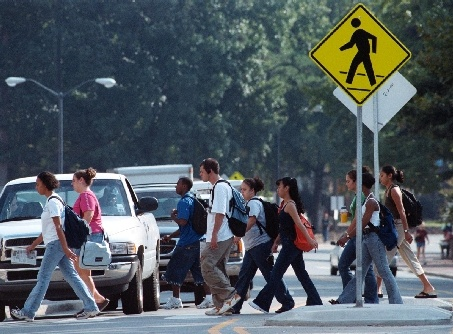
\includegraphics[width=5cm]{object_detection_image}}}%
%\qquad
%\subfloat[]{{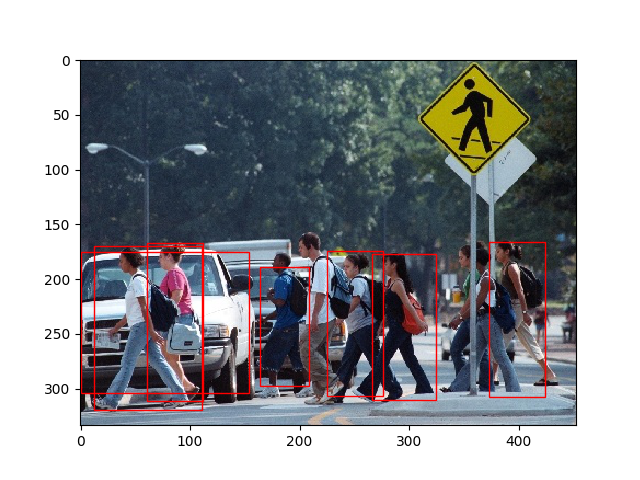
\includegraphics[width=6cm]{object_detection_boxes}}}%
%\caption{Imagen utilizada en el ejemplo. (b) muestra los cuadros delimitadores de lo objetos encontrados.}
%
%\end{figure}

\begin{sphinxVerbatim}[commandchars=\\\{\}]
\PYG{g+gp}{\PYGZgt{}\PYGZgt{}\PYGZgt{} }\PYG{k+kn}{from} \PYG{n+nn}{app}\PYG{n+nn}{.}\PYG{n+nn}{tf\PYGZus{}models}\PYG{n+nn}{.}\PYG{n+nn}{object\PYGZus{}detection} \PYG{k}{import} \PYG{n}{ObjectDetectionTensorflow}
\PYG{g+gp}{\PYGZgt{}\PYGZgt{}\PYGZgt{} }\PYG{n}{object\PYGZus{}detector} \PYG{o}{=} \PYG{n}{ObjectDetectionTensorflow}\PYG{p}{(}\PYG{p}{)}
\PYG{g+gp}{\PYGZgt{}\PYGZgt{}\PYGZgt{} }\PYG{n}{image\PYGZus{}base64} \PYG{o}{=} \PYG{l+s+s2}{\PYGZdq{}}\PYG{l+s+s2}{/9j/4AAQSkZJRgABAQEAYABgAAD/2...}\PYG{l+s+s2}{\PYGZdq{}}
\PYG{g+gp}{\PYGZgt{}\PYGZgt{}\PYGZgt{} }\PYG{n}{object\PYGZus{}detector}\PYG{o}{.}\PYG{n}{object\PYGZus{}detection}\PYG{p}{(}\PYG{n}{image\PYGZus{}base64}\PYG{p}{)}
\PYG{g+go}{[\PYGZob{}\PYGZsq{}confidence\PYGZsq{}: 0.8984639048576355, \PYGZsq{}category\PYGZsq{}: \PYGZsq{}car\PYGZsq{}, \PYGZsq{}topLeftY\PYGZsq{}: 175.0, \PYGZsq{}height\PYGZsq{}: 129.0, \PYGZsq{}width\PYGZsq{}: 154.0, \PYGZsq{}topLeftX\PYGZsq{}: 0.0\PYGZcb{},..., \PYGZob{}\PYGZsq{}confidence\PYGZsq{}: 0.6006952524185181, \PYGZsq{}category\PYGZsq{}: \PYGZsq{}person\PYGZsq{}, \PYGZsq{}topLeftY\PYGZsq{}: 189.0, \PYGZsq{}height\PYGZsq{}: 109.0, \PYGZsq{}width\PYGZsq{}: 45.0, \PYGZsq{}topLeftX\PYGZsq{}: 164.0\PYGZcb{}]}
\PYG{g+go}{\PYGZgt{}\PYGZgt{}\PYGZgt{}}
\end{sphinxVerbatim}



\codedocumentation{\sphinxbfcode{class }\sphinxcode{app.tf\_models.indoor\_scenes\_classifier.}\sphinxbfcode{ImageClassifier}}

Una clase pública que utiliza que utiliza una red neuronal
convolucional implementada en Tensorflow para clasificar en cuatro
clases una imagen. Las clases son:
desks,
exit,
office,
y soccer\_court.

Es la clase que carga el modelo ya entrenado, simplemente carga
la gráfica de cómputo que diseñamos con los parámetros
aprendidos. El clasificador puede
recibir una imagen codificada en base64 o su URL. El resultado
es un diccionario que pueda ser enviado como respuesta en la API
REST.

El siguiente ejemplo
muestra un simple uso de la clase. La imagen utilizada es la
de la figura \ref{fig:nao_soccer_court}
codificada en base 64.

\begin{figure}[htbp]
\centering
\caption{Cancha de entrenamiento del robot NAO.\label{fig:nao_soccer_court}}
\includegraphics[scale=0.3]{{soccer1}.jpg}
\end{figure}

\begin{sphinxVerbatim}[commandchars=\\\{\}]
\PYG{g+gp}{\PYGZgt{}\PYGZgt{}\PYGZgt{} }\PYG{k+kn}{from} \PYG{n+nn}{app}\PYG{n+nn}{.}\PYG{n+nn}{tf\PYGZus{}models}\PYG{n+nn}{.}\PYG{n+nn}{object\PYGZus{}detection} \PYG{k}{import} \PYG{n}{ImageClassifier}
\PYG{g+gp}{\PYGZgt{}\PYGZgt{}\PYGZgt{} }\PYG{n}{test\PYGZus{}image} \PYG{o}{=} \PYG{l+s+s2}{\PYGZdq{}}\PYG{l+s+s2}{/9j/4AAQSkZJRgABAQAAAQABAAD/2...}\PYG{l+s+s2}{\PYGZdq{}}
\PYG{g+gp}{\PYGZgt{}\PYGZgt{}\PYGZgt{} }\PYG{n}{clasifier} \PYG{o}{=} \PYG{n}{ImageClassifier}\PYG{p}{(}\PYG{p}{)}
\PYG{g+gp}{\PYGZgt{}\PYGZgt{}\PYGZgt{} }\PYG{n}{classifier}\PYG{o}{.}\PYG{n}{classify\PYGZus{}image}\PYG{p}{(}\PYG{n}{test\PYGZus{}image}\PYG{p}{)}
\PYG{g+go}{\PYGZob{}\PYGZsq{}indoor\PYGZus{}scene\PYGZsq{}: \PYGZsq{}soccer\PYGZus{}court\PYGZsq{}\PYGZcb{}}
\PYG{g+go}{\PYGZgt{}\PYGZgt{}\PYGZgt{}}
\end{sphinxVerbatim}

\subparagraph{Cliente de servicios web de terceros (\sphinxstyleemphasis{tpa\_client\_libraries})}
\label{\detokenize{chapter_two/desc_cloudnao:cliente-de-servicios-web-de-terceros-tpa-client-libraries}}\phantomsection\label{\detokenize{chapter_two/desc_cloudnao:module-app.tpa_client_libraries.google_cloud_translation}}\index{app.tpa\_client\_libraries.google\_cloud\_translation (módulo)}\index{GoogleCloudTranslation (clase en app.tpa\_client\_libraries.google\_cloud\_translation).}

En este paquete se encuentran los módulos para hacer las peticiones
a las API REST de los servicios en la nube de Google Cloud, Kairos
y Wit.ai.


\codedocumentation{\sphinxbfcode{class }\sphinxcode{app.tpa\_client\_libraries.google\_cloud\_translation.}\sphinxbfcode{GoogleCloudTranslation}}

Una clase pública que se conecta a la API de traducción de Google Cloud,
la cual permite traducir una cadena dada en un cualquier idioma admitido.
Hay tres métodos que provee la API; \sphinxcode{translate}, que recibe una cadena y
retorna su traducción, \sphinxcode{detect}, para detectar el idioma de un texto y
\sphinxcode{languages}, que retorna la lista de todos los idiomas disponibles para
la traducción.

El usado es \sphinxcode{translate}, a través de un \sphinxcode{POST} a
\sphinxcode{https://translation.googleapis.com/language/translate/v2}. El cuerpo
del mensaje HTTP debe tener al menos dos parámetros \sphinxcode{q} y \sphinxcode{target},
el texto de entrada y el código del lenguaje al que se traducirá el texto
de entrada, respectivamente.

En el siguiente fragmento de código en una terminal de Python interactiva
se muestra cómo utilizar este módulo.

\begin{sphinxVerbatim}[commandchars=\\\{\}]
\PYG{g+gp}{\PYGZgt{}\PYGZgt{}\PYGZgt{} }\PYG{k+kn}{from} \PYG{n+nn}{app}\PYG{n+nn}{.}\PYG{n+nn}{tpa\PYGZus{}client\PYGZus{}libraries}\PYG{n+nn}{.}\PYG{n+nn}{google\PYGZus{}cloud\PYGZus{}translation} \PYG{k}{import} \PYG{n}{GoogleCloudTranslation}
\PYG{g+gp}{\PYGZgt{}\PYGZgt{}\PYGZgt{} }\PYG{n}{translate} \PYG{o}{=} \PYG{n}{GoogleCloudTranslation}\PYG{p}{(}\PYG{p}{)}
\PYG{g+gp}{\PYGZgt{}\PYGZgt{}\PYGZgt{} }\PYG{n}{translate}\PYG{o}{.}\PYG{n}{translate}\PYG{p}{(}\PYG{l+s+s2}{\PYGZdq{}}\PYG{l+s+s2}{Cuervo, cuervo, no soporto más tu mirada}\PYG{l+s+s2}{\PYGZdq{}}\PYG{p}{,} \PYG{l+s+s2}{\PYGZdq{}}\PYG{l+s+s2}{en}\PYG{l+s+s2}{\PYGZdq{}}\PYG{p}{)}
\PYG{g+go}{\PYGZob{}\PYGZsq{}sourceLanguage\PYGZsq{}: \PYGZsq{}es\PYGZsq{}, \PYGZsq{}targetText\PYGZsq{}: \PYGZsq{}Crow, crow, I can not stand your gaze anymore\PYGZsq{}, \PYGZsq{}sourceText\PYGZsq{}: \PYGZsq{}Cuervo, cuervo, no soporto más tu mirada\PYGZsq{}\PYGZcb{}}
\PYG{g+go}{\PYGZgt{}\PYGZgt{}\PYGZgt{}}
\end{sphinxVerbatim}

\phantomsection\label{\detokenize{chapter_two/desc_cloudnao:module-app.tpa_client_libraries.google_cloud_vision}}\index{app.tpa\_client\_libraries.google\_cloud\_vision (módulo)}\phantomsection\label{\detokenize{chapter_two/desc_cloudnao:module-google_cloud_vision}}\index{google\_cloud\_vision (módulo)}\index{GoogleCloudVision (clase en app.tpa\_client\_libraries.google\_cloud\_vision)}


\codedocumentation{\sphinxbfcode{class }\sphinxcode{app.tpa\_client\_libraries.google\_cloud\_vision.}\sphinxbfcode{GoogleCloudVision}}

Una clase pública para integrar en la aplicación dos de las características
ofrecidas por Google Cloud Vision, el reconocimiento óptico de caracteres y
el etiquetado de imágenes, usando su API REST.

El recurso de la API de Google Cloud Vision utilizado es \sphinxcode{v1.images},
y la URL es
\sphinxcode{https://vision.googleapis.com/v1/images:annotate}. Por lo que hacer
un \sphinxcode{POST} al URL anterior ejecuta el procesamiento de un lote de imágenes.

El cuerpo del mensaje HTTP en la petición a la API de Google Cloud Vision,
debe tener la siguiente estructura.

\begin{sphinxVerbatim}[commandchars=\\\{\}]
\PYG{p}{\PYGZob{}}
  \PYG{l+s+s2}{\PYGZdq{}requests\PYGZdq{}}\PYG{o}{:} \PYG{p}{[}
    \PYG{p}{\PYGZob{}}
      \PYG{l+s+s2}{\PYGZdq{}features\PYGZdq{}}\PYG{o}{:} \PYG{p}{[}
        \PYG{p}{\PYGZob{}}
          \PYG{l+s+s2}{\PYGZdq{}type\PYGZdq{}}\PYG{o}{:} \PYG{l+s+s2}{\PYGZdq{}TEXT\PYGZus{}DETECTION\PYGZdq{}}
        \PYG{p}{\PYGZcb{}}\PYG{p}{,}
        \PYG{p}{\PYGZob{}}
          \PYG{l+s+s2}{\PYGZdq{}type\PYGZdq{}}\PYG{o}{:} \PYG{l+s+s2}{\PYGZdq{}LABEL\PYGZus{}DETECTION\PYGZdq{}}
        \PYG{p}{\PYGZcb{}}
      \PYG{p}{]}\PYG{p}{,}
      \PYG{l+s+s2}{\PYGZdq{}image\PYGZdq{}}\PYG{o}{:} \PYG{p}{\PYGZob{}}
        \PYG{l+s+s2}{\PYGZdq{}content\PYGZdq{}}\PYG{o}{:} \PYG{l+s+s2}{\PYGZdq{}\PYGZdq{}}\PYG{p}{,}
        \PYG{l+s+s2}{\PYGZdq{}source\PYGZdq{}}\PYG{o}{:} \PYG{p}{\PYGZob{}}
          \PYG{l+s+s2}{\PYGZdq{}imageUri\PYGZdq{}}\PYG{o}{:} \PYG{l+s+s2}{\PYGZdq{}\PYGZdq{}}
        \PYG{p}{\PYGZcb{}}
      \PYG{p}{\PYGZcb{}}
    \PYG{p}{\PYGZcb{}}
  \PYG{p}{]}
\PYG{p}{\PYGZcb{}}
\end{sphinxVerbatim}

En el parámetro \sphinxcode{features} solo añadimos las dos que utilizamos. El objeto
\sphinxcode{image} contiene la imagen que se desea analizar, y acepta la imagen codificada
en base64 (\sphinxcode{content}) o un URL (\sphinxcode{imageUri}).

Además de el cuerpo con la imagen es necesaria una API Key en los parámetros
del URL.

El siguiente ejemplo muestra un uso simple de esta clase cliente de la API
de Google Cloud.

\begin{sphinxVerbatim}[commandchars=\\\{\}]
\PYG{g+gp}{\PYGZgt{}\PYGZgt{}\PYGZgt{} }\PYG{k+kn}{from} \PYG{n+nn}{app}\PYG{n+nn}{.}\PYG{n+nn}{tpa\PYGZus{}client\PYGZus{}libraries}\PYG{n+nn}{.}\PYG{n+nn}{google\PYGZus{}cloud\PYGZus{}vision} \PYG{k}{import} \PYG{n}{GoogleCloudVision}
\PYG{g+gp}{\PYGZgt{}\PYGZgt{}\PYGZgt{} }\PYG{n}{vision} \PYG{o}{=} \PYG{n}{GoogleCloudVision}\PYG{p}{(}\PYG{p}{)}
\PYG{g+gp}{\PYGZgt{}\PYGZgt{}\PYGZgt{} }\PYG{n}{vision}\PYG{o}{.}\PYG{n}{text\PYGZus{}annotations\PYGZus{}description}\PYG{p}{(}\PYG{l+s+s1}{\PYGZsq{}}\PYG{l+s+s1}{https://new2.fjcdn.com/comments/Quote+from+this+scene+in+blade+runner+1982+dayum+son+\PYGZus{}fbf2a406e9c802ff492e414c34fff791.jpeg}\PYG{l+s+s1}{\PYGZsq{}}\PYG{p}{,} \PYG{k+kc}{True}\PYG{p}{)}
\PYG{g+go}{\PYGZob{}\PYGZsq{}text\PYGZsq{}: \PYGZsq{}You reach down and you flip the\PYGZbs{}ntortoise over on its back, Leon.\PYGZbs{}n\PYGZsq{}\PYGZcb{}}
\PYG{g+gp}{\PYGZgt{}\PYGZgt{}\PYGZgt{} }\PYG{n}{vision}\PYG{o}{.}\PYG{n}{label\PYGZus{}annotations\PYGZus{}description}\PYG{p}{(}\PYG{l+s+s1}{\PYGZsq{}}\PYG{l+s+s1}{https://new2.fjcdn.com/comments/Quote+from+this+scene+in+blade+runner+1982+dayum+son+\PYGZus{}fbf2a406e9c802ff492e414c34fff791.jpeg}\PYG{l+s+s1}{\PYGZsq{}}\PYG{p}{,} \PYG{k+kc}{True}\PYG{p}{)}
\PYG{g+go}{[\PYGZob{}\PYGZsq{}confidence\PYGZsq{}: 0.76214135, \PYGZsq{}name\PYGZsq{}: \PYGZsq{}photo caption\PYGZsq{}\PYGZcb{}, \PYGZob{}\PYGZsq{}confidence\PYGZsq{}: 0.569268, \PYGZsq{}name\PYGZsq{}: \PYGZsq{}film\PYGZsq{}\PYGZcb{}, \PYGZob{}\PYGZsq{}confidence\PYGZsq{}: 0.55112684, \PYGZsq{}name\PYGZsq{}: \PYGZsq{}screenshot\PYGZsq{}\PYGZcb{}]}
\PYG{g+go}{\PYGZgt{}\PYGZgt{}\PYGZgt{}}
\end{sphinxVerbatim}

\phantomsection\label{\detokenize{chapter_two/desc_cloudnao:module-app.tpa_client_libraries.kairos_client}}\index{app.tpa\_client\_libraries.kairos\_client (módulo)}\phantomsection\label{\detokenize{chapter_two/desc_cloudnao:module-kairos}}\index{kairos (módulo)}\index{Kairos (clase en app.tpa\_client\_libraries.kairos\_client)}

\codedocumentation{\sphinxbfcode{class }\sphinxcode{app.tpa\_client\_libraries.kairos\_client.}\sphinxbfcode{Kairos}}

Una clase pública que sirve como cliente para conectarse a dos servicios
que brinda la API de Kairos, el almacenamiento de rostros en una galería en la nube, y
la identificación de caras previamente guardadas.

Para ocupar estos servicios la API de Kairos provee los recursos \sphinxcode{enroll} y
\sphinxcode{recognize}, los cuales soportan el método \sphinxcode{POST} y tienen como
URL base \sphinxcode{http://api.kairos.com/}. Para hacer estas peticiones se
necesita una forma de autenticación, y esta es através de los encabezados
del mensaje HTTP, enviando en estos un id y una llave de la aplicación.

El cuerpo del \sphinxcode{POST} a \sphinxcode{recognize} tiene necesita al dos parámetros; la
imagen, que puede ser su URL o la codificación en base 64
y el nombre de la galería de donde de donde se desea identificar el rostro.

\begin{sphinxVerbatim}[commandchars=\\\{\}]
\PYG{p}{\PYGZob{}}
    \PYG{l+s+s2}{\PYGZdq{}image\PYGZdq{}} \PYG{o}{:} \PYG{l+s+s2}{\PYGZdq{}\PYGZdq{}}\PYG{p}{,}
    \PYG{l+s+s2}{\PYGZdq{}gallery\PYGZus{}name\PYGZdq{}} \PYG{o}{:} \PYG{l+s+s2}{\PYGZdq{}\PYGZdq{}}
\PYG{p}{\PYGZcb{}}
\end{sphinxVerbatim}

El cuerpo del \sphinxcode{POST} a {enroll} requiere de al menos tres argumentos;
la imagen, el nombre de la galería y el identificador del rostro, que
comúnmente es el nombre de la persona con esa cara.

\begin{sphinxVerbatim}[commandchars=\\\{\}]
\PYG{p}{\PYGZob{}}
    \PYG{l+s+s2}{\PYGZdq{}image\PYGZdq{}} \PYG{o}{:} \PYG{l+s+s2}{\PYGZdq{}\PYGZdq{}}\PYG{p}{,}
    \PYG{l+s+s2}{\PYGZdq{}subject\PYGZus{}id\PYGZdq{}} \PYG{o}{:} \PYG{l+s+s2}{\PYGZdq{}\PYGZdq{}}\PYG{p}{,}
    \PYG{l+s+s2}{\PYGZdq{}gallery\PYGZus{}name\PYGZdq{}} \PYG{o}{:} \PYG{l+s+s2}{\PYGZdq{}\PYGZdq{}}
\PYG{p}{\PYGZcb{}}
\end{sphinxVerbatim}

Un ejemplo del uso del módulo.

\begin{sphinxVerbatim}[commandchars=\\\{\}]
\PYG{g+gp}{\PYGZgt{}\PYGZgt{}\PYGZgt{} }\PYG{k+kn}{from} \PYG{n+nn}{app}\PYG{n+nn}{.}\PYG{n+nn}{tpa\PYGZus{}client\PYGZus{}libraries}\PYG{n+nn}{.}\PYG{n+nn}{kairos\PYGZus{}client} \PYG{k}{import} \PYG{n}{Kairos}
\PYG{g+gp}{\PYGZgt{}\PYGZgt{}\PYGZgt{} }\PYG{n}{face} \PYG{o}{=} \PYG{n}{Kairos}\PYG{p}{(}\PYG{p}{)}
\PYG{g+gp}{\PYGZgt{}\PYGZgt{}\PYGZgt{} }\PYG{n}{face}\PYG{o}{.}\PYG{n}{enroll}\PYG{p}{(}\PYG{l+s+s2}{\PYGZdq{}}\PYG{l+s+s2}{http://www.indiewire.com/wp\PYGZhy{}content/uploads/2017/10/triboro\PYGZus{}build03.jpeg?w=780}\PYG{l+s+s2}{\PYGZdq{}}\PYG{p}{,} \PYG{l+s+s2}{\PYGZdq{}}\PYG{l+s+s2}{Rachael}\PYG{l+s+s2}{\PYGZdq{}}\PYG{p}{)}
\PYG{g+go}{\PYGZob{}\PYGZsq{}faceEnroll\PYGZsq{}: \PYGZob{}\PYGZsq{}gender\PYGZsq{}: \PYGZsq{}M\PYGZsq{}, \PYGZsq{}width\PYGZsq{}: 235, \PYGZsq{}topLeftY\PYGZsq{}: 232, \PYGZsq{}confidence\PYGZsq{}: 0.99931, \PYGZsq{}height\PYGZsq{}: 235, \PYGZsq{}topLeftX\PYGZsq{}: 232\PYGZcb{}\PYGZcb{}}
\PYG{g+gp}{\PYGZgt{}\PYGZgt{}\PYGZgt{} }\PYG{n}{face}\PYG{o}{.}\PYG{n}{recognize}\PYG{p}{(}\PYG{l+s+s2}{\PYGZdq{}}\PYG{l+s+s2}{https://i.ytimg.com/vi/j4jIJB8c1I8/maxresdefault.jpg}\PYG{l+s+s2}{\PYGZdq{}}\PYG{p}{)}
\PYG{g+go}{\PYGZob{}\PYGZsq{}faceRecognize\PYGZsq{}: \PYGZob{}\PYGZsq{}subject\PYGZus{}id\PYGZsq{}: \PYGZsq{}Rachael\PYGZsq{}, \PYGZsq{}width\PYGZsq{}: 342, \PYGZsq{}topLeftY\PYGZsq{}: 165, \PYGZsq{}confidence\PYGZsq{}: 0.63092, \PYGZsq{}height\PYGZsq{}: 342, \PYGZsq{}topLeftX\PYGZsq{}: 366\PYGZcb{}\PYGZcb{}}
\PYG{g+go}{\PYGZgt{}\PYGZgt{}\PYGZgt{}}
\end{sphinxVerbatim}


\phantomsection\label{\detokenize{chapter_two/desc_cloudnao:module-app.tpa_client_libraries.wit_api}}\index{app.tpa\_client\_libraries.wit\_api (módulo)}\phantomsection\label{\detokenize{chapter_two/desc_cloudnao:module-wit_api}}\index{wit\_api (módulo)}\index{WitAPI (clase en app.tpa\_client\_libraries.wit\_api)}


\codedocumentation{\sphinxbfcode{class }\sphinxcode{app.tpa\_client\_libraries.wit\_api.}\sphinxbfcode{WitAPI}}

Una clase pública donde se hacen las peticiones HTTP
a Wit.ai y para extraer el significado del audio o texto. Funciona como
un módulo cliente para solicitar los recursos de \sphinxcode{/message} y \sphinxcode{/speech}.
Estos recursos tiene la función de hallar información estructurada dentro
de una oración.

En seguida se muestra cómo utilizar el método \sphinxcode{message()} para
enlistar las entidades encontradas en una cadena de texto.

\begin{sphinxVerbatim}[commandchars=\\\{\}]
\PYG{g+gp}{\PYGZgt{}\PYGZgt{}\PYGZgt{} }\PYG{k+kn}{from} \PYG{n+nn}{app}\PYG{n+nn}{.}\PYG{n+nn}{tpa\PYGZus{}client\PYGZus{}libraries}\PYG{n+nn}{.}\PYG{n+nn}{wit\PYGZus{}api} \PYG{k}{import} \PYG{n}{WitAPI}
\PYG{g+gp}{\PYGZgt{}\PYGZgt{}\PYGZgt{} }\PYG{n}{wit\PYGZus{}example} \PYG{o}{=} \PYG{n}{WitAPI}\PYG{p}{(}\PYG{p}{)}
\PYG{g+gp}{\PYGZgt{}\PYGZgt{}\PYGZgt{} }\PYG{n}{wit\PYGZus{}example}\PYG{o}{.}\PYG{n}{message}\PYG{p}{(}\PYG{l+s+s2}{\PYGZdq{}}\PYG{l+s+s2}{Lee el texto de esta fotografía}\PYG{l+s+s2}{\PYGZdq{}}\PYG{p}{)}
\PYG{g+go}{\PYGZob{}\PYGZsq{}textDetect\PYGZsq{}: [\PYGZob{}\PYGZsq{}confidence\PYGZsq{}: 0.76588128565519, \PYGZsq{}type\PYGZsq{}: \PYGZsq{}value\PYGZsq{}, \PYGZsq{}value\PYGZsq{}: \PYGZsq{}lee\PYGZsq{}\PYGZcb{}, \PYGZob{}\PYGZsq{}confidence\PYGZsq{}: 0.95853105168152, \PYGZsq{}type\PYGZsq{}: \PYGZsq{}value\PYGZsq{}, \PYGZsq{}value\PYGZsq{}: \PYGZsq{}texto\PYGZsq{}\PYGZcb{}], \PYGZsq{}photography\PYGZsq{}: [\PYGZob{}\PYGZsq{}confidence\PYGZsq{}: 0.65220641878769, \PYGZsq{}type\PYGZsq{}: \PYGZsq{}value\PYGZsq{}, \PYGZsq{}value\PYGZsq{}: \PYGZsq{}fotografía\PYGZsq{}\PYGZcb{}]\PYGZcb{}}
\PYG{g+go}{\PYGZgt{}\PYGZgt{}\PYGZgt{}}
\end{sphinxVerbatim}
\index{message() (método de app.tpa\_client\_libraries.wit\_api.WitAPI)}


\subparagraph{Utilidades (\sphinxstyleemphasis{utils})}
\label{\detokenize{chapter_two/desc_cloudnao:utilidades-utils}}\index{make\_request() (en el módulo app.utils.requests\_utils)}

Este paquete incluye funciones auxiliares
para hacer peticiones HTTP utilizando la biblioteca 
\texttt{requests} de Python, funciones para validar
la autenticación y cargar una imagen en un arreglo
de \texttt{numpy}.


\paragraph{Configuración y ejecución}
\label{\detokenize{chapter_two/desc_cloudnao:configuracion-y-ejecucion}}
La aplicación cuenta con varias opciones de configuración, principalmente
para \sphinxcode{SQLAlchemy} y para activar el debugging durante la ejecución.

Para la ejecución de la aplicación simplemente se corre el
script \sphinxstyleemphasis{manage.py}. Eligiendo ya sea la interfaz de línea de comandos:

\begin{sphinxVerbatim}[commandchars=\\\{\}]
\PYGZdl{} python manage.py shell
\end{sphinxVerbatim}

O lanzar el servidor:

\begin{sphinxVerbatim}[commandchars=\\\{\}]
\PYGZdl{} python manage.py runserver
\end{sphinxVerbatim}


\subparagraph{config.py}
\label{\detokenize{chapter_two/desc_cloudnao:config-py}}\label{\detokenize{chapter_two/desc_cloudnao:module-config}}\index{config (módulo)}
Programa que establece las opciones de configuración para la
aplicación.
\index{Config (clase en config)}


\subparagraph{manage.py}
\label{\detokenize{chapter_two/desc_cloudnao:module-manage}}\label{\detokenize{chapter_two/desc_cloudnao:manage-py}}\index{manage (módulo)}
El programa que inicia la aplicación.
\index{create\_tables() (en el módulo manage)}

